\chapter{Optimization Using Mathematical Programs with Complementarity Constraints} \label{cap:optimization_mpcc}

This chapter presents an optimization approach based on Mathematical Programs with Complementarity Constraints (MPCC) to address the natural gas transportation problem, with a particular focus on modeling the nonlinear behavior of gas flow in pipelines governed by the Weymouth equation. The MPCC framework offers a mathematical structure for incorporating the nonconvexities and discontinuities inherent in gas network models, thereby enabling a more precise representation of the underlying physical constraints. This methodology is relevant in scenarios involving the interconnection between natural gas and electrical systems, where operational decisions in one network directly influence the other. The results presented in this chapter have been peer-reviewed and published in an article featured in an A1-ranked journal according to the PUBLINDEX classification.

\section{Formulation of Interconnected Power and Gas Systems} \label{sec:formulation}


An interconnected system can be effectively represented by a directed graph denoted as $ G = \left\lbrace\mathcal{N}, \mathcal{E}\right\rbrace$, where the sets of units $\mathcal{N}$ and edges $\mathcal{E}$ consider all power and gas components along with their interconnections. On the electrical power side, the system holds power units $\mathcal{N}_P\subset\mathcal{N}$, termed buses, and power edges $\mathcal{B}\subset\mathcal{E}$ or branches. The power buses comprise generators $\mathcal{G}\subset\mathcal{N}_P$ injecting power and users $\mathcal{D}\subset\mathcal{N}_P$ demanding power~\cite{WANG2019113410}. The branches $\mathcal{B} = \left\{b=(n,m) \mid n,m\in\mathcal{N}_P \right\}$ connect the buses to make the electrical power flow from the generators to the users. Although the physical power flow is alternating current, the system is accurately modeled using a linear direct current (DC) approximation. The DC model ignores reactive power flows and voltage magnitude fluctuations and approximates active power flows using linear transfer distribution factors~\cite{DC_flow}. Further, the linear characteristics allow stating linear programming problems. Thus, the DC model serves as an appropriate approximation for many power system operations and planning studies, providing a balance of accuracy and computational tractability~\cite{DC_flow2}. 

Then, the optimization problem of the interconnected system seeks to minimize the operation costs for satisfying the demands of the interconnected system while encompassing the power and gas constraints. Specifically, the following cost function linearly combines the flows of power and gas through the operation costs of the interconnected system elements:

\begin{equation} \label{eq:obj_func_integrated}
\begin{split}
\min_{\mathcal{P}, \mathcal{F}} \quad  \sum_{g \in \mathcal{G}} C_{g}^t {P_{g}^t} + \sum_{d \in \mathcal{D}} C_{d}^t {P_{d}^t} +  \sum_{w \in \mathcal{W}} C_{w}^t {f_{w}^t} + \\ \sum_{p \in \mathcal{P}} C_{p}^t {f_{p}^t}  + \sum_{c \in \mathcal{C}} C_{c}^t {f_{c}^t} + \sum_{u \in \mathcal{U}} C_{u}^{t} {f_{u}^{t}} + \\ \quad \sum_{s \in \mathcal{S}} C_{s+}^{t} {f_{s+}^{t}}  + \sum_{s \in \mathcal{S}} C_{s-}^{t} {f_{s-}^{t}} + \sum_{s \in \mathcal{S}} C_{s}^{t} {V_{s}^{t}}
\end{split}
\end{equation}

\noindent where $C_g^t$ denotes the generation cost by the $g$-th bus and $C_d^t$ the unsupplied power demand for the $d$-th user. Regarding the natural gas system, terms $C_w^t$, $C_p^t$, $C_c^t$ and $C_u^t$ are the same as those used in \Cref{eq:obj_func_linear_gas}. However, some additional terms are considered in this case: $C_{s+}^t$, $C_{s-}^t$, and $C_{s}^t$ represent the costs of injecting, extracting, and storing gas at the $s$-th storage station.

Therefore, the decision variables for the optimization problem are $P_g^t$ for the generated power, $P_d^t$ for the unsupplied power, $f_w^t$ for the inject gas flow, $f_p^t$ and $f_c^t$ for the transported gas through pipeline $p$ and compressor $c$, $f_u^t$ for the unsupplied gas demand, $f_{s+}^t$, $f_{s-}^t$, and $f_{s}^t$ for injecting, extracting, and storing gas. Traditionally, a transported gas with a positive value of $ f_ { p } ^t>0 $ moves in the predefined direction, while a negative value flows in the opposite one, with no impact on the optimization process. On the other hand, compressor stations solely allow unidirectional gas flow, expressed as $f_{c}^t\geq0$. By optimizing this integrated cost function while adhering to the system's operational constraints, the proposed methodology effectively balances the demands of both energy systems, leading to a comprehensive solution that minimizes costs while ensuring reliable and efficient operation.

Optimization of the integrated cost function in \Cref{eq:obj_func_integrated} while adhering to the system's operational constraints must lead to a comprehensive solution balancing the demands of both energy systems while ensuring reliable and efficient operation. Three sets of operational constraints describe the within and between power and gas interplay.

The first constraint set guarantees a stable power system operation: \Cref{eq:gen_limits} ensures that the generated power $P_{g}^t$ lies between the technical minimum $\underline{P_g^t}$ and maximum $\overline{P_g^t}$. \Cref{eq:line_limits} bounds the power flow through the transmission line $P_{l}^t$, preventing damages, such as overheating. \Cref{eq:dc_power_flow} models the power flow over the electrical network through the reactance-based relationship of the power flow $P_{l}^t$, the line susceptance $B_{nm}$, and the voltage angles $\theta_n,\theta_{m}$ at buses $n,m$. \Cref{eq:dem_limit_power} limits the unsupplied power $P_{d}^t$ to the user demand $\overline{P_{d}^t}$. \Cref{eq:voltage_angle_limits} ensures stable operating conditions within the interconnected power grid by restricting the bus voltage angles. \Cref{eq:power_balance} defines the power balance at each bus, i.e., the total input and generated power must equal the total output and unsupplied power, being $\mathcal{B}_{n+}=\{(m,n')\in\mathcal{B}:n'=n\}$ and $\mathcal{B}_{n-}=\{(n',m)\in\mathcal{B}:n'=n\}$ the set of inflow and outflow transmission lines at the $n$-th bus, respectively.

\begin{alignat}{4}
    \underline{P_g^t} \leq P_{g}^t \leq \overline{P_g^t} &\quad \forall \ g \in \mathcal{G}, \label{eq:gen_limits} \\
    -\overline{P_l^t} \leq P_{l}^t \leq \overline{P_l^t} &\quad \forall \ l \in \mathcal{L}, \label{eq:line_limits} \\
    P_{l}^t = B_{nm}(\theta_n - \theta_{m}) &\quad \forall \ l = (n, m) \in \mathcal{L} , \label{eq:dc_power_flow} \\
    0 \leq P_{d}^t \leq \overline{P_{d}^t} &\quad \forall \ d \in \mathcal{D}, \label{eq:dem_limit_power} \\
    -\overline{\theta_{n}^t} \leq \theta_{n}^t \leq \overline{\theta_{n}^t} &\quad \forall \ n \in \mathcal{N}_P, \label{eq:voltage_angle_limits} \\
    \sum_{\substack{l\in \mathcal{B}_{n+}\\g=n}}{P_{l}^t + P_{g}^t} = \sum_{\substack{l\in \mathcal{B}_{n-}\\d=n}} P_{l}^t + P_{d}^t &\quad \forall \ n \in \mathcal{N}_P \label{eq:power_balance} 
    % + \sum\limits_{n \in \mathcal{G}} P_{n}^t - \sum\limits_{n \in \mathcal{D}} P_{n}^t = 0 \quad \forall \ n,m \in \mathcal{N}_P \label{eq:power_balance} 
\end{alignat}
% \end{subequations}

The second constraint set interconnects natural gas and electrical power systems through gas-fired power plants generating electricity, as expressed by \Cref{eq:gas_power_relation} , where $f_{n}^t$ stands for the natural gas fuel consumption to generate a power $P_{n}^t$ at generator bus $n\in\mathcal{N}_I$, the heat-rate $\text{HR}_n$ defines the generator efficiency, and the set $\mathcal{N}_I=\mathcal{G}\cap\mathcal{U}$ holds all thermoelectrical plants as the gas users that generate power.

\begin{align}
    &f_{n}^t = P_{n}^t \cdot \text{HR}_n, \quad \forall \ n \in \mathcal{N}_I, \label{eq:gas_power_relation} 
\end{align}

The third constraint set models the gas transportation system: Besides \Cref{eq:well_limits,eq:pipe_limits,eq:dem_limit_gas,eq:gas_balance}, \Cref{eq:press_limit} fixes safe operating limits for the pressure on the $n$-th node $\pi_{n}^t$ as $[\underline{\pi_{n}^t},\overline{\pi_{n}^t}]$. The constraint in \Cref{eq:comp_ratio} asserts that the compression ratio $\pi_{m}^t / \pi_{n}^t$ cannot physically exceed the compressor's design limitation  $\beta_{c}\geq1 \ \forall c=(n,m) \in \mathcal{C}$, enabling the representation of different compressors by adjusting the values of $\beta_{c}\geq1$.  \Cref{eq:sto_limit1,eq:sto_limit2} limit the gas injection $f_{s+}^t$  and extraction $f_{s-}^t$ rates at storage facilities according to the feasible operating range determined by the currently stored volume $V_{s}^t$, respectively. In turn, \Cref{eq:sto_time} balances the gas storage unit such that gas volume at operation period $t$, $V_{s}^t$, equals the volume from period $V_{s}^{t-1}$ plus the difference between injected $f_{s+}^{t-1}$ and extracted $f_{s+}^{t-1}$ gas flow; a fundamental constraint for modeling the dynamics of gas storage over time. Lastly, \Cref{eq:weymouth_constraint}, known as the Weymouth equation, summarizes the physical behavior of gas flow through pipelines by relating the gas flow through the pipeline $f_{p}^t$ to the pressures at the ends of the pipeline $\pi_{n}^t, \pi_{m}^t \ \forall \ p = (n,m) \in\mathcal{P}$. The constant $K_{nm}$ in this equation is a pipeline-specific coefficient that encapsulates various physical characteristics, including its length, diameter, and friction factor, as well as the properties of the gas being transported. The Weymouth equation defines a nonlinear, nonconvex, disjunctive flow-pressure relationship that hampers the optimization of the gas transport system.


\begin{alignat}{4}
    \underline{\pi_{n}^t} \leq \pi_{n}^t \leq \overline{\pi_{n}^t} &\quad \forall \ n \in \mathcal{N}_f, \quad \forall \ t \in T \label{eq:press_limit} \\
    \pi_{m}^t \leq \beta_{c}^t{\pi_{n}^t} &\quad \forall c=(n,m) \in \mathcal{C}, \quad \forall \ t \in T \label{eq:comp_ratio} \\
    0 \leq f_{s+}^t \leq V_{0s} - \underline{V_s} &\quad \forall \ s \in \mathcal{S} , \quad \forall \ t \in T \label{eq:sto_limit1} \\ 
    0 \leq f_{s-}^t \leq \overline{V_s} - V_{0s} &\quad \forall \ s \in \mathcal{S}, \quad \forall \ t \in T \label{eq:sto_limit2} \\ 
    V_{s}^t = V_{s}^{t-1} + f_{s-}^{t-1} - f_{s+}^{t-1} &\quad \forall \ s \in \mathcal{S}, \quad \forall \ t \in T \label{eq:sto_time}\\
    sgn(f_{p}^t)(f_{p}^t)^2 = K_{nm}((\pi_{n}^t)^2-(\pi_{m}^t)^2) &\quad \forall \ p =(n,m) \in\mathcal{P}, \quad \forall \ t \in T \label{eq:weymouth_constraint}
\end{alignat}


\section{Mathematical Programming with Complementarity Constraints for Weymouth Approximation} \label{sec:mpcc}

The Weymouth equation is the fundamental model for gas flow through pipelines. Nevertheless, it presents a challenge for optimal interconnected operation due to its nonlinearity, which arises from the signum function determining the gas flow direction. This nonlinearity results from the complex physics of gas flow, making it challenging to find optimal solutions for gas transportation systems~\citep{weymouth_nonconvex}. Traditional optimization methods have difficulties in solving the nonconvexity of the Weymouth equation. However, recent advances in optimization techniques, particularly mathematical programs with complementary constraints (MPCC), offer a solution to address this issue. MPCC specializes in handling complementarity constraints and non-convexities, making it well-suited to tackle the intricacies of the Weymouth equation~\citep{baumrucker_renfro_biegler_2008}. This type of formulation involves optimization problems of the general form:


\begin{subequations}
\begin{alignat}{4}
\mathcal{O}: \ &\min \ q(x, y) \\
&\text{s.t. } h_i(x, y) = 0 \\
&\quad g_j(x, y) \geq 0 \\
&\quad 0 \leq G_k(x) \perp H_k(y) \geq 0 \label{eq:complementarity}
\end{alignat}
\end{subequations}



% where $f(x, y) \in \mathbb{R}$ is the cost function, and $x$ and $y$ represent vectors of optimization variables. Specifically, $x$ often contains variables related to the primal optimization problem, and $y$ typically contains variables associated with the optimality conditions or complementary relationships, which may include Lagrange multipliers or auxiliary variables from the inner problem in bilevel optimization. The functions $h(x,y) \in \mathbb{R}^{N_h}$ and $g(x,y) \in \mathbb{R}^{N_g}$ capture equality and inequality constraints in the optimization problem $\mathcal{O}$, respectively. The sub-index $i$ enumerates the equality constraints, with a total of $N_h$ such constraints, while the sub-index $j$ enumerates the inequality constraints, with a total of $N_g$ such constraints. 



\noindent Here, \( x \in \mathbb{R}^n \) and \( y \in \mathbb{R}^m \) are the decision variables, typically representing primal and dual components, or system and auxiliary variables, respectively. The objective function \( q(x, y) \in \mathbb{R} \) is to be minimized, subject to a set of equality constraints \( h_i(x, y) = 0 \) for all \( i \in \mathcal{z} \), where \( |\mathcal{z}| \) denotes the number of such constraints, and a set of inequality constraints \( g_j(x, y) \geq 0 \) for all \( j \in \mathcal{R} \), with \( |\mathcal{R}| \) indicating the number of inequality constraints. The complementarity conditions in~\Cref{eq:complementarity} involve mappings \( G_k: \mathbb{R}^n \to \mathbb{R} \) and \( H_k: \mathbb{R}^m \to \mathbb{R} \), defined for all \( k \in \mathcal{K} \), where \( |\mathcal{K}| \) is the total number of complementarity pairs. The notation \( 0 \leq G_k(x) \perp H_k(y) \geq 0 \) expresses the condition that for each \( k \in \mathcal{K} \), the product \( G_k(x) \cdot H_k(y) = 0 \), with both terms being non-negative. This ensures that at least one element in each complementarity pair is zero at the optimum, thereby modeling the disjunctive or switching behavior characteristic of gas flow through pipelines.

% where $f(x, y)$ is the cost function, $h(x,y)$ and $g(x,y)$ capture equality and inequality constraints in the optimization problem $\mathcal{O}$. \Cref{eq:complementarity} represents the complementarity conditions, with the operator $\perp$ indicating that at a solution, either $x$ or $y$ must be zero while the other must remain non-negative. These conditions turn MPCC into a modeling tool for scenarios with variables exhibiting complementarity relationships, such as economic equilibrium~\citep{MPCC_advantages}, variational inequalities~\citep{Hintermüller_Kopacka_2009}, and the intricate dynamics of natural gas transportation systems~\citep{Hante_Schmidt_2019}.
To deal with the non-convexity, this work rewrites the Weymouth equation as the following mathematical program with two complementarity constraints:
\begin{alignat}{4}
\label{eq:complementarity_relaxec3}
\mathcal{O}_W: \ &\min\limits_{y_p^t} -y_p^tf_{p}^t \\
& \text{s.t. } y_p^t(f_{p}^t)^2 = K_{nm}((\pi_{n}^t)^2-(\pi_{m}^t)^2)\nonumber\\
& -1 \leq y_p^t \leq 1 \nonumber\\
&f_{p}^t = f_{p+}^t - f_{p-}^t\nonumber\\
& 0 \leq f_{p+}^t \perp (y_p^t+1) \geq 0 \nonumber\\
& 0 \leq f_{p-}^t \perp (1-y_p^t) \geq 0 \nonumber
\end{alignat}
where $f_{p+}^t\geq0$ and $f_{p-}^t\geq0$ hold the positive and negative components of the gas flow in the $p$-th pipeline at operation period $t$, for assessing directional flow.


In problem $\mathcal{O}_W$, the objective function minimizes the product $-y_p^t f_p^t$, which promotes alignment between the direction of gas flow and its magnitude, as defined by the auxiliary variable $y_p^t \in [-1,1]$. The first constraint in $\mathcal{O}_W$ enforces the Weymouth relationship in its relaxed form, where the product $y_p^t (f_p^t)^2$ equals the pressure drop across the pipeline scaled by the constant $K_{nm}$, such that $K_{nm}((\pi_n^t)^2 - (\pi_m^t)^2)$ captures the non-linear physics of gas flow between nodes $n$ and $m$ at time $t$. The second constraint bounds the direction variable $y_p^t$ between $-1$ and $1$, allowing it to encode bidirectional flow while keeping the model numerically stable. The third constraint defines the net gas flow $f_p^t$ as the difference between its non-negative forward and reverse components, $f_{p+}^t$ and $f_{p-}^t$, respectively. 

The final two constraints are complementarity conditions: $0 \leq f_{p+}^t \perp (y_p^t + 1) \geq 0$ and $0 \leq f_{p-}^t \perp (1 - y_p^t) \geq 0$. These conditions enforce that the gas can only flow in one direction at a time. Specifically, if $f_{p+}^t > 0$, then $y_p^t = -1$, indicating flow from node $m$ to node $n$, while if $f_{p-}^t > 0$, then $y_p^t = 1$, indicating flow in the opposite direction. This formulation allows the MPCC to capture the switching behavior of gas flows due to changes in pressure direction, without resorting to discrete variables or binary decision-making.

Solving MPCC presents a unique set of challenges distinguishing it from traditional optimization problems. One notable challenge is the need for regularity properties, making MPCC more complex~\citep{MPCC_lack_properties}. Compared to smooth optimization problems, where gradients and Hessians provide valuable information for optimization algorithms, MPCC often lacks these properties, leading to difficulties in devising efficient numerical methods.

% \subsection{Linear Independence Constraint Qualification (LICQ)}
%
% The Linear Independence Constraint Qualification (LICQ) is a critical condition in optimization, particularly in nonlinear programming problems (NLPs). LICQ ensures the existence and uniqueness of Lagrange multipliers, simplifying their interpretation and enhancing the clarity of their role in constrained optimization. Additionally, LICQ provides a robust framework for local analysis, guaranteeing that the KKT conditions are sufficient for optimality when satisfied at a specific point.~\citep{Bergmann_Herzog_2019}.
%
% LICQ is a constraint qualification used in optimization problems to ensure that the gradients of the active inequality constraints and the gradients of the equality constraints are linearly independent at the minimizing point $x^{*}$ of the original constrained optimization problem $\mathcal{P}$, understanding the set of active constraints as, 
%
% \begin{equation} \label{eq:active_inequalities}
%     I(x^*) := \left \{1 \leq l \leq p \,|\, g_l(x^*) = 0\right \}, 
% \end{equation}
% i.e., the inequality constraints at the point $x^{*}$ that lie on its boundary. The above indicates that this constraint qualification is fulfilled when the elements of the set $\mathcal{F}$ are linearly independent at the point $x^{*}$.
%
% \begin{equation} \label{eq: LICQ }
%      \mathcal{F} = \{ (\nabla h_1(x^*)), \ldots, (\nabla h_m(x^*)), (\nabla g_n(x^*), \, \forall n \in I(x^*)) \}    
% \end{equation}
%
% \subsection{Mangasarian-Fromovitz Constraint Qualification (MFCQ)}
%
% When an optimization problem does not meet the LICQrequirements, it is possible to resort to a second,less stringent criterion to check whether the KKT conditions are satisfied. This second criterion is known as Mangasarian-Fromovitz Constraint Qualification (MFCQ). The LICQ focuses on ensuring linear independence of the gradients of the active inequality and equality constraints~\citep{BertsekasDimitriP1999Np/D}. On the other hand, the main objective of MFCQ is to guarantee that the gradients of the equality constraints are linearly independent at the optimal point $\mathbf{x}^*$, and furthermore that there exists a vector $\mathbf{d} \in \mathbb{R}^n$ such that
%
%  \begin{equation}
%     \nabla h_i(\mathbf{x}^*)^\top \mathbf{d} < 0    
%  \end{equation}
%   
% for all equality constraints.
%
%
% \begin{equation}
%     \nabla g_j(\mathbf{x}^*)^\top \mathbf{d} < 0    
% \end{equation}
%
% and for all active inequality constraints.  
 

It is widely recognized that conventional constraint qualifications in nonlinear programming, such as LICQ and MFCQ, are typically not satisfied in the case of MPCC. As a result, KKT conditions commonly associated with MPCC may not be applicable or valid at a local minimization point~\citep{Bouza_Still_2007}. Therefore, posing relaxed nonlinear programs (RNLP)  deals with the numerical resolution of MPCC by introducing a positive regularization parameter $\epsilon\in\mathbb{R}^+$ that simplifies the solution and properly handles the inequalities~\citep{Scholtes_2001}. These programs typically satisfy constraint qualifications, making them more amenable to efficient optimization techniques. Relaxing MPCC ensures that inequalities are appropriately treated as inactive, particularly when $G_k(x)H_k(y) \leq \epsilon$, enhancing their structural integrity. Besides, relaxed programs  reliably approximate the original problem as $\epsilon\to0$~\citep{Scheel_Scholtes_2000}. Hence, instead of working with the original problem $\mathcal{O}_W$ as can be seen in \Cref{eq:complementarity_relaxec3}, the relaxed problem $\mathcal{O}_\epsilon$ is formulated:


\begin{subequations}
\begin{alignat}{4}
\label{eq:complementarity_relaxec1}
\mathcal{O}_\epsilon: \ &\min\limits_{y_p^t} -y_p^tf_{p}^t \\
&\text{s.t. } y_p^t(f_{p}^t)^2 = K_{nm}((\pi_{n}^t)^2-(\pi_{m}^t)^2)\\
&f_{p}^t = f_{p+}^t - f_{p-}^t\\
& -1 \leq y_p^t \leq 1 \\
&\quad f_{p+}^t(y_p^t+1) \leq \epsilon\label{eq:Oe:complementarity1} \\ \label{eq:Oe:complementarity2}
&\quad f_{p-}^t(1-y_p^t) \leq \epsilon
\end{alignat}
\end{subequations}


Theoretically, the relaxed problem offers fundamental properties that tackle challenging MPCC problems~\citep{Ralph_Wright_2004}. Firstly, the relaxed approach guarantees the convergence to the true MPCC solution as $\epsilon\to0$. Additionally, the boundedness of Lagrange multipliers ensures numerical stability and avoids issues with infinitely large values during optimization. Lastly, the local uniqueness of the $\mathcal{O}_{\epsilon}$ solution under specific conditions guarantees a single and well-defined solution. Therefore, the proposed relaxed optimization problem deals with the non-convexity in the Weymouth equation while guaranteeing the KKT conditions around $\epsilon$, posing a standard optimization problem, and avoiding ambiguity in interpreting results.

\section{Case studies} \label{sec:case_study}
The current section validates the proposed MPCC approach by comparing its performance against two well-established methods for approximating the Weymouth equation: i) The Taylor series approach that piecewise approximates Weymouth with line segments~\cite{ORDOUDIS2019642} and ii) The SOC programming that introduces a two-stage optimization, namely, flow direction estimation and cost minimization~\cite{soc_paper}. 

The validation aims to quantify the inherent errors and the relationship between cost and error in the contrasted approaches to support their real-world pertinence. Therefore, this work reports two performance metrics: the cost function in \Cref{eq:obj_func_integrated} that assesses the capacity for optimally operating an integrated system and the Weymouth error metric (${WE}_p^t\in\mathbb{R}^+$) for quantifying the required flow to guarantee equality for pipeline $p$ at time instant $t$ in~\Cref{eq:weymouth_cons}:
\begin{equation}
    {WE}_p^t = \left|f_{p}^t - \left(K_{nm}|(\pi_{n}^t)^2-(\pi_{m}^t)^2|\right)^{1/2}\right| , \quad \forall \ p =(n,m) \in\mathcal{P}.
    \label{eq:weymouth_cons}
\end{equation}

\noindent Hence, the ${WE}_p^t$ metric, measured in million standard cubic feet per day (MMSCFD), explains the approximations' inherent sensitivity and validates the significance of their differences. The validation contrasts Taylor, SOC, and MPCC approaches in three case studies of interconnected systems with different complexities.

\subsection{Case Study I: 9/8 System}


The network depicted in \Cref{fig:8-9 network}~\cite{Wilson_poly} interconnects a nine-bus power system and an eight-node natural gas network. The small size of case 9/8 enables fast execution, efficient analysis, and rigorous validation of the contrasted approaches. The 9/8 network also features a closed trajectory and bidirectional pipelines, allowing looped infrastructure with potential flow reversals.

\begin{figure}[H]
    \centering
    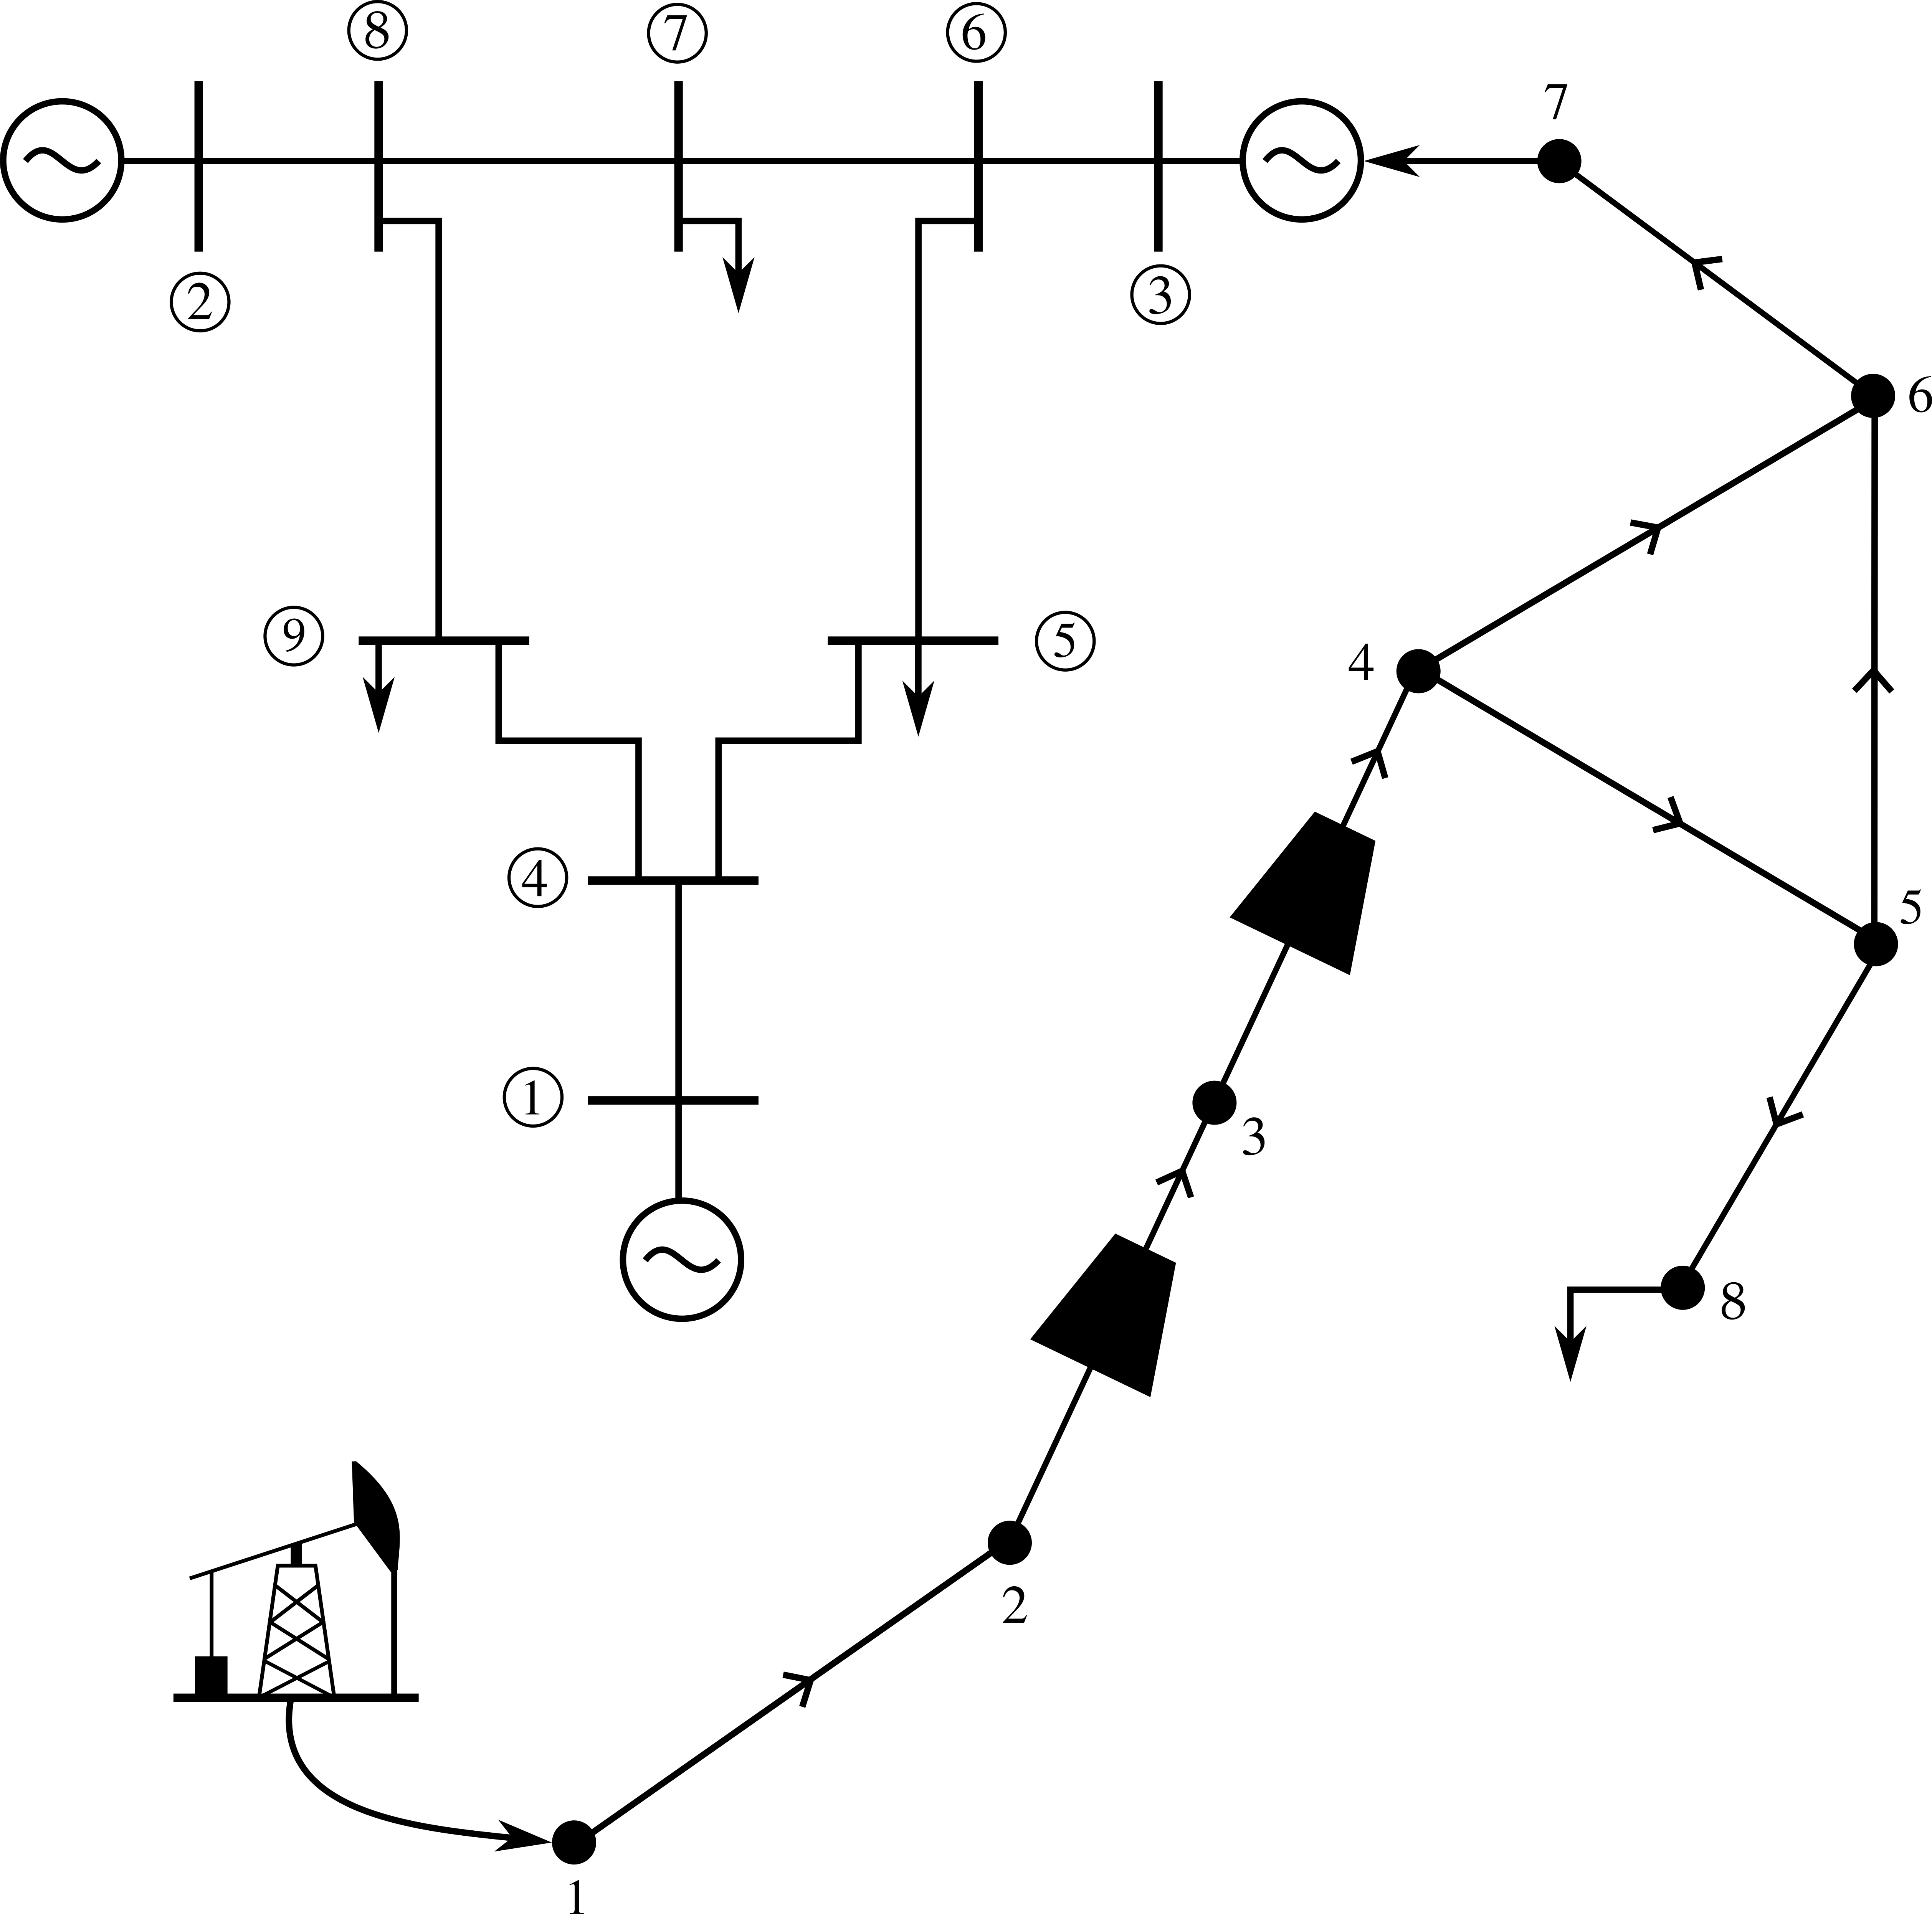
\includegraphics[scale=0.7]{figures/Chapter_MPCC/8 node 9 bus network.png}
    \caption{Integrated system 9/8 used in Case Study I, modified from the MATPOWER-NATURAL GAS (MPNG) software.}
    \label{fig:8-9 network}
\end{figure}

To assess the performance of Weymouth approximation approaches on the 9/8 system, a Monte Carlo experiment estimates the cost function and Weymouth error distributions by solving the optimization problem for one day ($\mathcal{T}=\left\lbrace 1\right\rbrace$) one hundred times with uniformly sampled natural gas demands. Further network parameter details can be found in the publicly available repository OptiGasFlow ({\url{https://github.com/cblancom/optigasflow}}, accessed on 05 April 2024). 
 \Cref{fig:blue_test_cost} depicts the cost function histogram for Taylor, SOC, and MPCC approaches. Remarkably, the three histograms evidence identical distribution patterns, leading to regular solutions across approaches.

The boxplots in~\Cref{fig:blue_test_boxplot} show the Weymouth approximation error distribution for each pipeline using three approaches. The error distributions, including median and interquartile range, indicate that MPCC consistently maintains accuracy throughout the network. In contrast, the widely varying errors of the Taylor and SOC approaches suggest a lack of consistency in the achieved solution. Therefore, in a small network, the proposed MPCC approach converges to identical operational costs as Taylor and SOC, even in rationing, while meeting all linear constraints and improving the Weymouth approximation.


\begin{figure}[H]
    \centering
    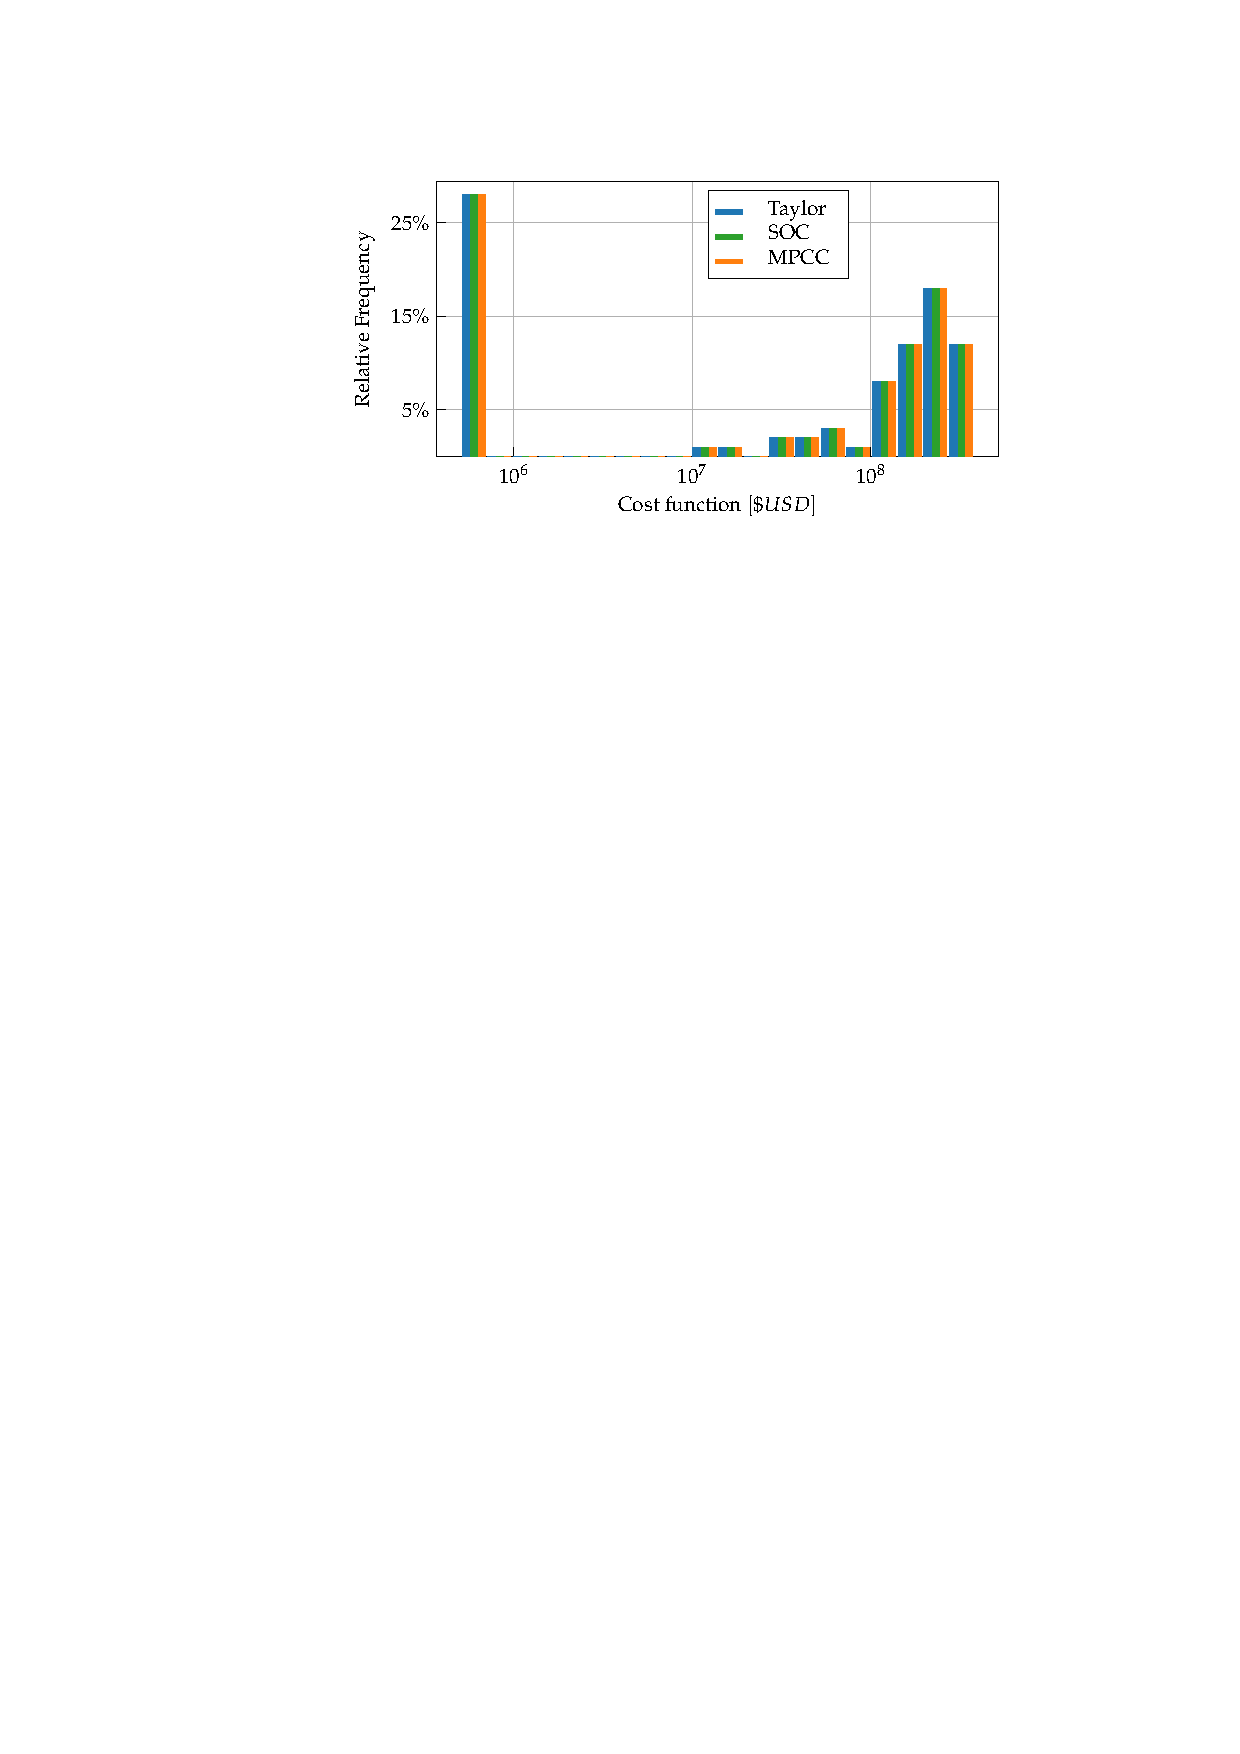
\includegraphics[scale=1]{figures/Chapter_MPCC/g001.pdf}
    % % This file was created with tikzplotlib v0.10.1.
\begin{tikzpicture}

\definecolor{darkgray176}{RGB}{176,176,176}
\definecolor{darkorange25512714}{RGB}{0,0,255}%{255,127,14}
% \definecolor{red}{RGB}{255,0,0}%{44,160,44}
\definecolor{lightgray204}{RGB}{204,204,204}
\definecolor{steelblue31119180}{RGB}{0,128,0}%{31,119,180}

\definecolor{red}{RGB}{255,127,14}
\definecolor{darkorange25512714}{RGB}{44,160,44}
\definecolor{steelblue31119180}{RGB}{31,119,180}
% \definecolor{darkgray176}{RGB}{176,176,176}
% \definecolor{darkorange25512714}{RGB}{255,127,14}
% \definecolor{green}{RGB}{0,128,0}

\begin{axis}[
width=\figurewidth,
height=\figureheight,
legend cell align={left},
legend style={fill opacity=0.8, draw opacity=1, text opacity=1, draw=lightgray204},
tick align=inside,
tick pos=left,
x grid style={darkgray176},
xlabel={Objective function cost},
xmin=5.56829803705899, xmax=8.71309423956304,
xtick style={color=black},
xtick={6,7,8},
xticklabels={
  \(\displaystyle {10^{6}}\),
  \(\displaystyle {10^{7}}\),
  \(\displaystyle {10^{8}}\),
},
xmajorgrids,
y grid style={darkgray176},
ymajorgrids,
ylabel=Relative Frequency,
ymin=0, ymax=29.4,
ytick style={color=black},
ytick={5,15,25},
yticklabels={
  \(\displaystyle {5\%}\),
  \(\displaystyle {15\%}\),
  \(\displaystyle {25\%}\),
},
]
\draw[draw=red,fill=red,fill opacity=0.75,line width=0.195771585198722pt] (axis cs:5.79744147894999,0) rectangle (axis cs:5.84054055892949,28);
\draw[draw=red,fill=red,fill opacity=0.75,line width=0.195771585198722pt] (axis cs:5.94110507888165,0) rectangle (axis cs:5.98420415886115,0);
\draw[draw=red,fill=red,fill opacity=0.75,line width=0.195771585198722pt] (axis cs:6.08476867881331,0) rectangle (axis cs:6.12786775879281,0);
\draw[draw=red,fill=red,fill opacity=0.75,line width=0.195771585198722pt] (axis cs:6.22843227874497,0) rectangle (axis cs:6.27153135872447,0);
\draw[draw=red,fill=red,fill opacity=0.75,line width=0.195771585198722pt] (axis cs:6.37209587867663,0) rectangle (axis cs:6.41519495865613,0);
\draw[draw=red,fill=red,fill opacity=0.75,line width=0.195771585198722pt] (axis cs:6.51575947860829,0) rectangle (axis cs:6.55885855858779,0);
\draw[draw=red,fill=red,fill opacity=0.75,line width=0.195771585198722pt] (axis cs:6.65942307853996,0) rectangle (axis cs:6.70252215851945,0);
\draw[draw=red,fill=red,fill opacity=0.75,line width=0.195771585198722pt] (axis cs:6.80308667847162,0) rectangle (axis cs:6.84618575845111,0);
\draw[draw=red,fill=red,fill opacity=0.75,line width=0.195771585198722pt] (axis cs:6.94675027840328,0) rectangle (axis cs:6.98984935838278,0);
\draw[draw=red,fill=red,fill opacity=0.75,line width=0.195771585198722pt] (axis cs:7.09041387833494,0) rectangle (axis cs:7.13351295831444,1);
\draw[draw=red,fill=red,fill opacity=0.75,line width=0.195771585198722pt] (axis cs:7.2340774782666,0) rectangle (axis cs:7.2771765582461,1);
\draw[draw=red,fill=red,fill opacity=0.75,line width=0.195771585198722pt] (axis cs:7.37774107819826,0) rectangle (axis cs:7.42084015817776,0);
\draw[draw=red,fill=red,fill opacity=0.75,line width=0.195771585198722pt] (axis cs:7.52140467812992,0) rectangle (axis cs:7.56450375810942,2);
\draw[draw=red,fill=red,fill opacity=0.75,line width=0.195771585198722pt] (axis cs:7.66506827806158,0) rectangle (axis cs:7.70816735804108,2);
\draw[draw=red,fill=red,fill opacity=0.75,line width=0.195771585198722pt] (axis cs:7.80873187799324,0) rectangle (axis cs:7.85183095797274,3);
\draw[draw=red,fill=red,fill opacity=0.75,line width=0.195771585198722pt] (axis cs:7.9523954779249,0) rectangle (axis cs:7.9954945579044,1);
\draw[draw=red,fill=red,fill opacity=0.75,line width=0.195771585198722pt] (axis cs:8.09605907785656,0) rectangle (axis cs:8.13915815783606,8);
\draw[draw=red,fill=red,fill opacity=0.75,line width=0.195771585198722pt] (axis cs:8.23972267778822,0) rectangle (axis cs:8.28282175776772,12);
\draw[draw=red,fill=red,fill opacity=0.75,line width=0.195771585198722pt] (axis cs:8.38338627771988,0) rectangle (axis cs:8.42648535769938,18);
\draw[draw=red,fill=red,fill opacity=0.75,line width=0.195771585198722pt] (axis cs:8.52704987765154,0) rectangle (axis cs:8.57014895763104,12);
\draw[draw=darkorange25512714,fill=darkorange25512714,fill opacity=0.75,line width=0.195771585198722pt] (axis cs:5.75434239897049,0) rectangle (axis cs:5.79744147894999,28);
\draw[draw=darkorange25512714,fill=darkorange25512714,fill opacity=0.75,line width=0.195771585198722pt] (axis cs:5.89800599890215,0) rectangle (axis cs:5.94110507888165,0);
\draw[draw=darkorange25512714,fill=darkorange25512714,fill opacity=0.75,line width=0.195771585198722pt] (axis cs:6.04166959883381,0) rectangle (axis cs:6.08476867881331,0);
\draw[draw=darkorange25512714,fill=darkorange25512714,fill opacity=0.75,line width=0.195771585198722pt] (axis cs:6.18533319876548,0) rectangle (axis cs:6.22843227874497,0);
\draw[draw=darkorange25512714,fill=darkorange25512714,fill opacity=0.75,line width=0.195771585198722pt] (axis cs:6.32899679869714,0) rectangle (axis cs:6.37209587867663,0);
\draw[draw=darkorange25512714,fill=darkorange25512714,fill opacity=0.75,line width=0.195771585198722pt] (axis cs:6.4726603986288,0) rectangle (axis cs:6.51575947860829,0);
\draw[draw=darkorange25512714,fill=darkorange25512714,fill opacity=0.75,line width=0.195771585198722pt] (axis cs:6.61632399856046,0) rectangle (axis cs:6.65942307853996,0);
\draw[draw=darkorange25512714,fill=darkorange25512714,fill opacity=0.75,line width=0.195771585198722pt] (axis cs:6.75998759849212,0) rectangle (axis cs:6.80308667847162,0);
\draw[draw=darkorange25512714,fill=darkorange25512714,fill opacity=0.75,line width=0.195771585198722pt] (axis cs:6.90365119842378,0) rectangle (axis cs:6.94675027840328,0);
\draw[draw=darkorange25512714,fill=darkorange25512714,fill opacity=0.75,line width=0.195771585198722pt] (axis cs:7.04731479835544,0) rectangle (axis cs:7.09041387833494,1);
\draw[draw=darkorange25512714,fill=darkorange25512714,fill opacity=0.75,line width=0.195771585198722pt] (axis cs:7.1909783982871,0) rectangle (axis cs:7.2340774782666,1);
\draw[draw=darkorange25512714,fill=darkorange25512714,fill opacity=0.75,line width=0.195771585198722pt] (axis cs:7.33464199821876,0) rectangle (axis cs:7.37774107819826,0);
\draw[draw=darkorange25512714,fill=darkorange25512714,fill opacity=0.75,line width=0.195771585198722pt] (axis cs:7.47830559815042,0) rectangle (axis cs:7.52140467812992,2);
\draw[draw=darkorange25512714,fill=darkorange25512714,fill opacity=0.75,line width=0.195771585198722pt] (axis cs:7.62196919808208,0) rectangle (axis cs:7.66506827806158,2);
\draw[draw=darkorange25512714,fill=darkorange25512714,fill opacity=0.75,line width=0.195771585198722pt] (axis cs:7.76563279801374,0) rectangle (axis cs:7.80873187799324,3);
\draw[draw=darkorange25512714,fill=darkorange25512714,fill opacity=0.75,line width=0.195771585198722pt] (axis cs:7.9092963979454,0) rectangle (axis cs:7.9523954779249,1);
\draw[draw=darkorange25512714,fill=darkorange25512714,fill opacity=0.75,line width=0.195771585198722pt] (axis cs:8.05295999787706,0) rectangle (axis cs:8.09605907785656,8);
\draw[draw=darkorange25512714,fill=darkorange25512714,fill opacity=0.75,line width=0.195771585198722pt] (axis cs:8.19662359780873,0) rectangle (axis cs:8.23972267778822,12);
\draw[draw=darkorange25512714,fill=darkorange25512714,fill opacity=0.75,line width=0.195771585198722pt] (axis cs:8.34028719774039,0) rectangle (axis cs:8.38338627771988,18);
\draw[draw=darkorange25512714,fill=darkorange25512714,fill opacity=0.75,line width=0.195771585198722pt] (axis cs:8.48395079767205,0) rectangle (axis cs:8.52704987765154,12);
\draw[draw=steelblue31119180,fill=steelblue31119180,fill opacity=0.75,line width=0.195771585198722pt] (axis cs:5.71124331899099,0) rectangle (axis cs:5.75434239897049,28);
\draw[draw=steelblue31119180,fill=steelblue31119180,fill opacity=0.75,line width=0.195771585198722pt] (axis cs:5.85490691892266,0) rectangle (axis cs:5.89800599890215,0);
\draw[draw=steelblue31119180,fill=steelblue31119180,fill opacity=0.75,line width=0.195771585198722pt] (axis cs:5.99857051885432,0) rectangle (axis cs:6.04166959883381,0);
\draw[draw=steelblue31119180,fill=steelblue31119180,fill opacity=0.75,line width=0.195771585198722pt] (axis cs:6.14223411878598,0) rectangle (axis cs:6.18533319876548,0);
\draw[draw=steelblue31119180,fill=steelblue31119180,fill opacity=0.75,line width=0.195771585198722pt] (axis cs:6.28589771871764,0) rectangle (axis cs:6.32899679869714,0);
\draw[draw=steelblue31119180,fill=steelblue31119180,fill opacity=0.75,line width=0.195771585198722pt] (axis cs:6.4295613186493,0) rectangle (axis cs:6.4726603986288,0);
\draw[draw=steelblue31119180,fill=steelblue31119180,fill opacity=0.75,line width=0.195771585198722pt] (axis cs:6.57322491858096,0) rectangle (axis cs:6.61632399856046,0);
\draw[draw=steelblue31119180,fill=steelblue31119180,fill opacity=0.75,line width=0.195771585198722pt] (axis cs:6.71688851851262,0) rectangle (axis cs:6.75998759849212,0);
\draw[draw=steelblue31119180,fill=steelblue31119180,fill opacity=0.75,line width=0.195771585198722pt] (axis cs:6.86055211844428,0) rectangle (axis cs:6.90365119842378,0);
\draw[draw=steelblue31119180,fill=steelblue31119180,fill opacity=0.75,line width=0.195771585198722pt] (axis cs:7.00421571837594,0) rectangle (axis cs:7.04731479835544,1);
\draw[draw=steelblue31119180,fill=steelblue31119180,fill opacity=0.75,line width=0.195771585198722pt] (axis cs:7.1478793183076,0) rectangle (axis cs:7.1909783982871,1);
\draw[draw=steelblue31119180,fill=steelblue31119180,fill opacity=0.75,line width=0.195771585198722pt] (axis cs:7.29154291823926,0) rectangle (axis cs:7.33464199821876,0);
\draw[draw=steelblue31119180,fill=steelblue31119180,fill opacity=0.75,line width=0.195771585198722pt] (axis cs:7.43520651817092,0) rectangle (axis cs:7.47830559815042,2);
\draw[draw=steelblue31119180,fill=steelblue31119180,fill opacity=0.75,line width=0.195771585198722pt] (axis cs:7.57887011810258,0) rectangle (axis cs:7.62196919808208,2);
\draw[draw=steelblue31119180,fill=steelblue31119180,fill opacity=0.75,line width=0.195771585198722pt] (axis cs:7.72253371803424,0) rectangle (axis cs:7.76563279801374,3);
\draw[draw=steelblue31119180,fill=steelblue31119180,fill opacity=0.75,line width=0.195771585198722pt] (axis cs:7.86619731796591,0) rectangle (axis cs:7.9092963979454,1);
\draw[draw=steelblue31119180,fill=steelblue31119180,fill opacity=0.75,line width=0.195771585198722pt] (axis cs:8.00986091789756,0) rectangle (axis cs:8.05295999787706,8);
\draw[draw=steelblue31119180,fill=steelblue31119180,fill opacity=0.75,line width=0.195771585198722pt] (axis cs:8.15352451782923,0) rectangle (axis cs:8.19662359780873,12);
\draw[draw=steelblue31119180,fill=steelblue31119180,fill opacity=0.75,line width=0.195771585198722pt] (axis cs:8.29718811776089,0) rectangle (axis cs:8.34028719774039,18);
\draw[draw=steelblue31119180,fill=steelblue31119180,fill opacity=0.75,line width=0.195771585198722pt] (axis cs:8.44085171769255,0) rectangle (axis cs:8.48395079767205,12);


\node[draw,fill=white,anchor=north east] at (axis description cs:0.735,0.97) {
    \begin{tabular}{@{}cl}
        \tikz\draw[steelblue31119180,fill=steelblue31119180] (0,0) rectangle (15,5); & Taylor \\
        \tikz\draw[darkorange25512714,fill=darkorange25512714] (0,0) rectangle (15,5); & SOC \\
        \tikz\draw[red,fill=red] (0,0) rectangle (15,5); & MPCC \\
    \end{tabular}
};

\end{axis}

\end{tikzpicture}

    \caption{Cost function histogram for the Taylor, SOC, and MPCC Weymouth approximation approaches in the 9-bus 8-node system.}
    \label{fig:blue_test_cost}
\end{figure}

\vspace{-10pt}
\begin{figure}[H]
    
     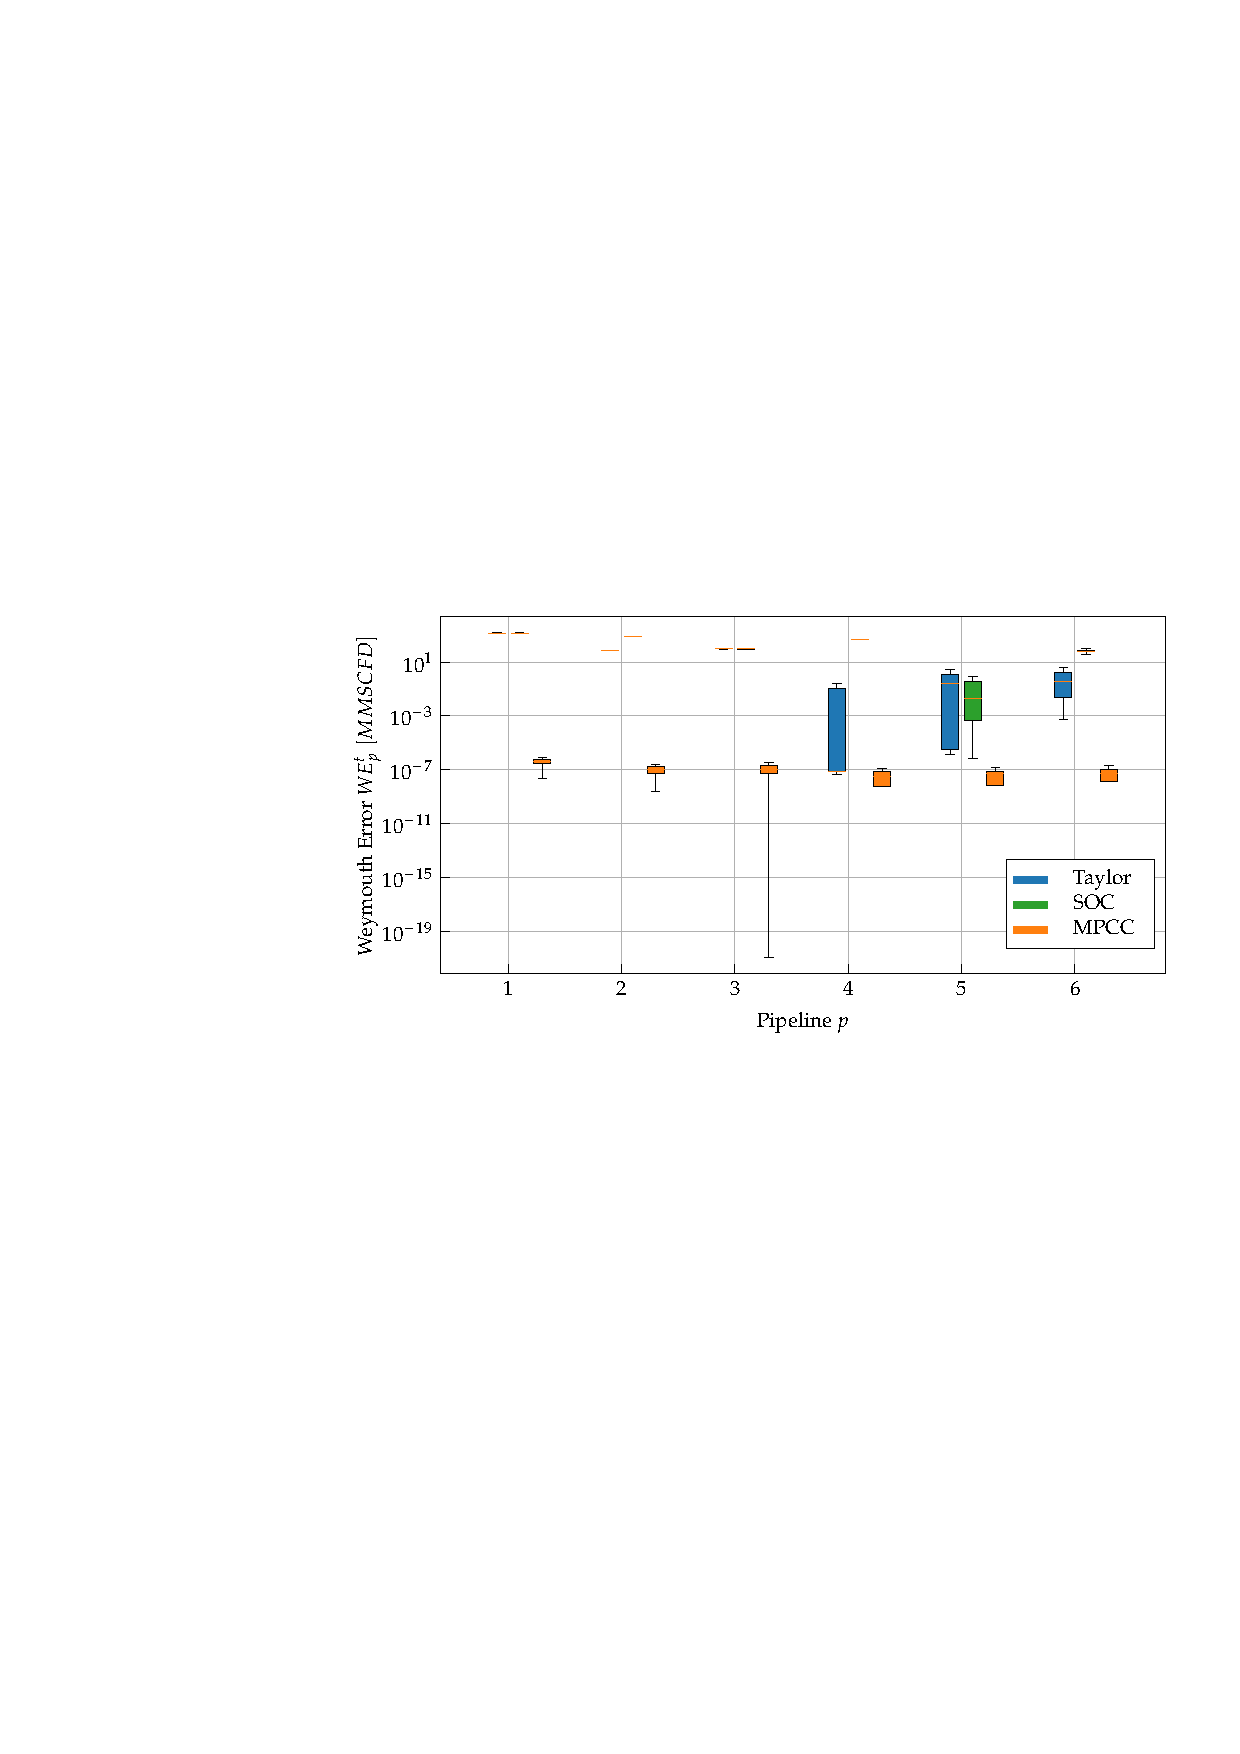
\includegraphics[scale=0.98]{figures/Chapter_MPCC/g002.pdf}
    \caption{Boxplot of Weymouth error distribution for each pipeline in the 9/8 system attained by contrasted approximation approaches.}
    \label{fig:blue_test_boxplot}
\end{figure}

\subsection{Case II: 118/48 System}

The following case simulates a complex, large-scale electric grid system, the widely studied IEEE 118 bus system~\citep{WANG201970}, consisting of 54 generator buses, 9 fed by the gas system, 186 transmission lines, and 99 users, that is, $\left| \mathcal{G} \right| = 54, \left| \mathcal{F} \right| = 186, \left| \mathcal{D} \right| = 99$. This electric grid interconnects with a 48-node natural gas system featuring 9 supply wells, 46 pipelines, eight compressor stations, and 22 user nodes through 9 connection points, i.e., $\left| \mathcal{W} \right| = 9, \left| \mathcal{P} \right| = 46, \left| \mathcal{C} \right| = 8, \left| \mathcal{U} \right| = 22, \left| \mathcal{I} \right| = 9$~\citep{Conejo}. The network topology deliberately introduces closed flow loops to stress the solver and the constraint approximations, as do real-world systems.

\Cref{fig:green_test_cost} depicts the histogram of relative cost differences for the MPCC proposal to Taylor and SOC baselines from a hundred trials of the Monte Carlo experiment and a considered operation of one day ($T=1$). It is worth noting that both baselines yielded the same cost function values. The relative difference between MPCC and the baselines is always positive, indicating that the complementarity constraint formulation consistently produces larger cost values in this system. However, the maximum difference of 6\% falls within the range of real-world variations due to the dispatcher's practical decisions in line with the actual pressure--flow relationship~\citep{ZHAO2023129010}. 

\begin{figure}[H]
    \centering
    
   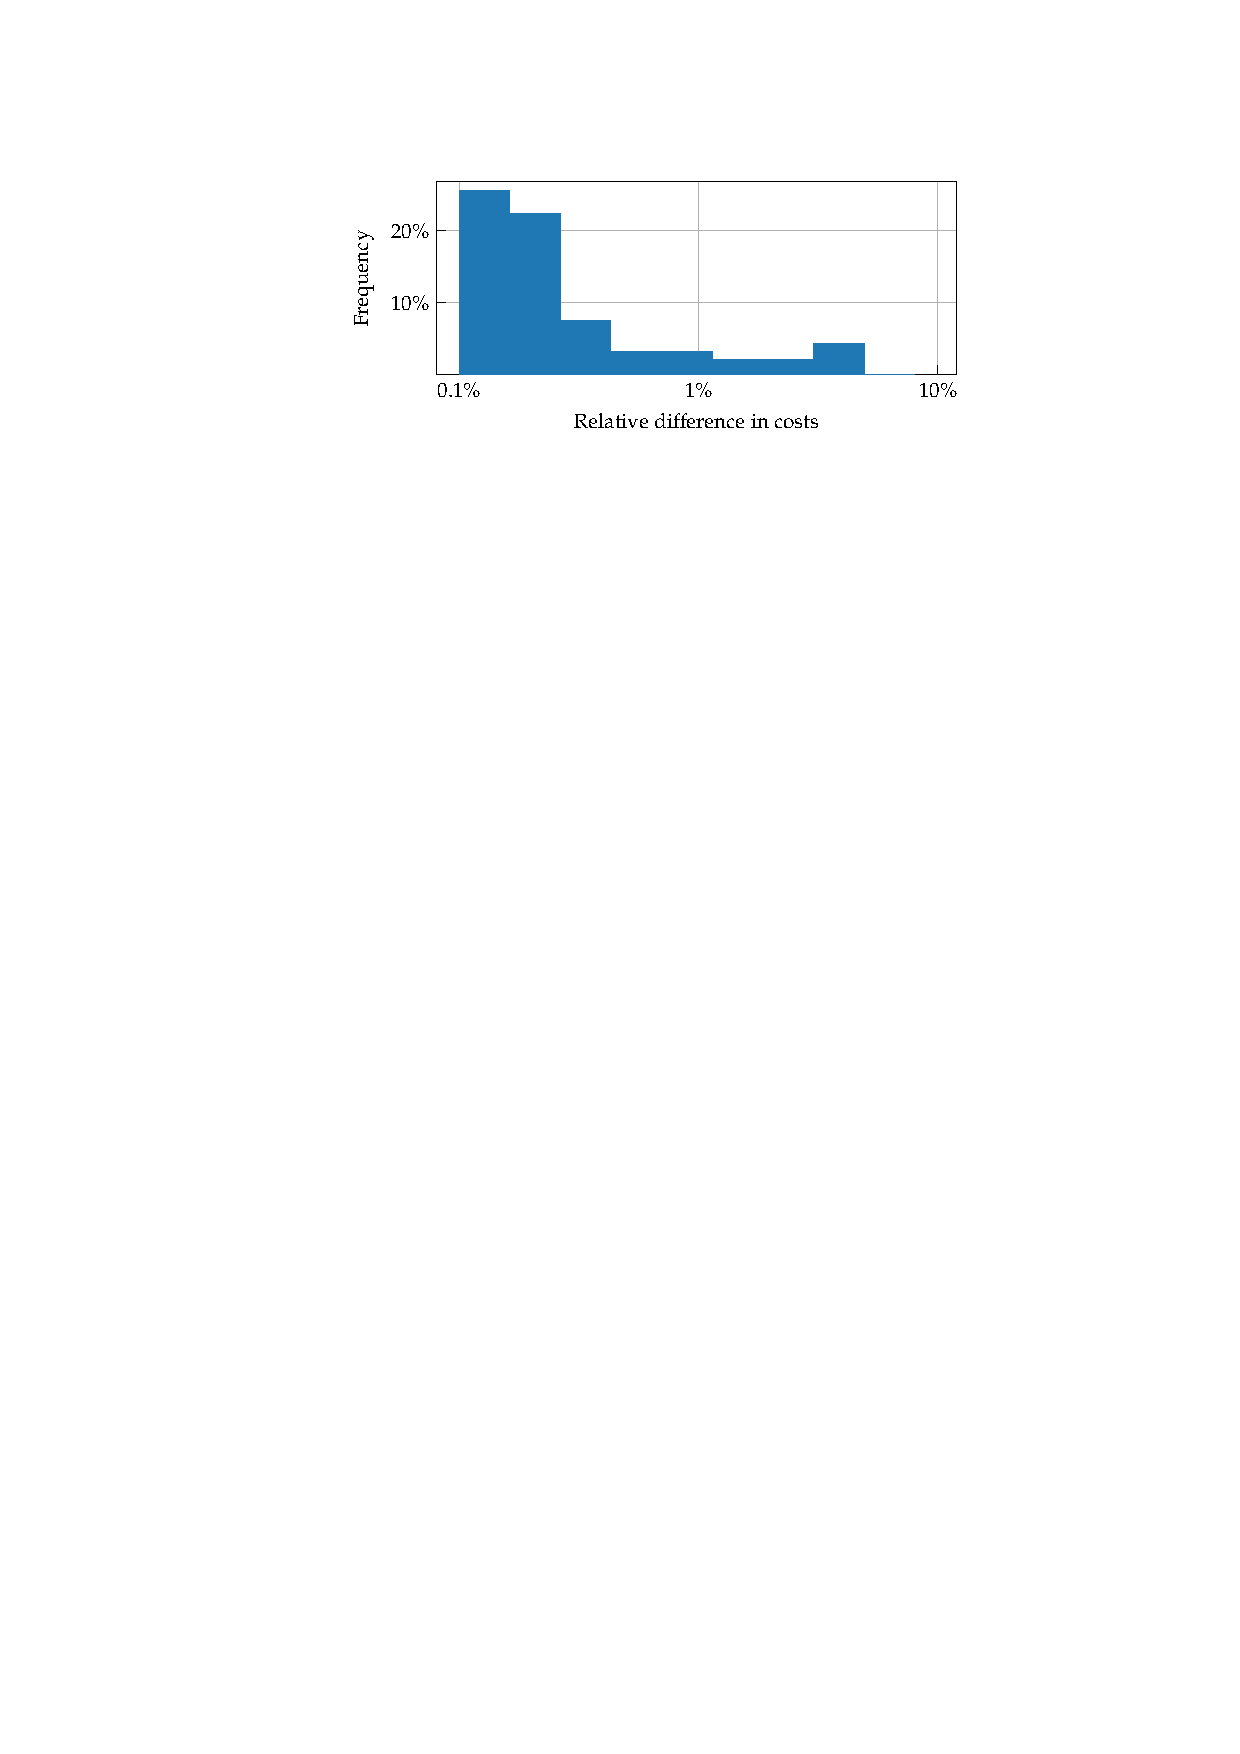
\includegraphics[scale=1]{figures/Chapter_MPCC/g003.pdf}
    \caption{Histogram depicting the relative frequencies of cost differences obtained between MPCC and the other approaches in the 48-node 118-bus system.}
    \label{fig:green_test_cost}
\end{figure}

Contrarily to cost function analysis, results in \Cref{fig:green_test_error} reveal a significant error reduction of about seven orders of magnitude (from $10^1$ to $10^{-6}$) under the proposed complementarity constraints. As an additional benefit, MPCC exhibits a shorter error dispersion than Taylor and SOC at most of the 46 pipelines in the network. Such behavior in the 118/48 system, also evidenced in the small 9/8 case study, proves the reliability of MPCC in effectively addressing more complex network configurations and interconnected dynamics.


\vspace{-6pt}
\begin{figure}[H]
% \begin{adjustwidth}{-\extralength}{0cm}
\centering    
    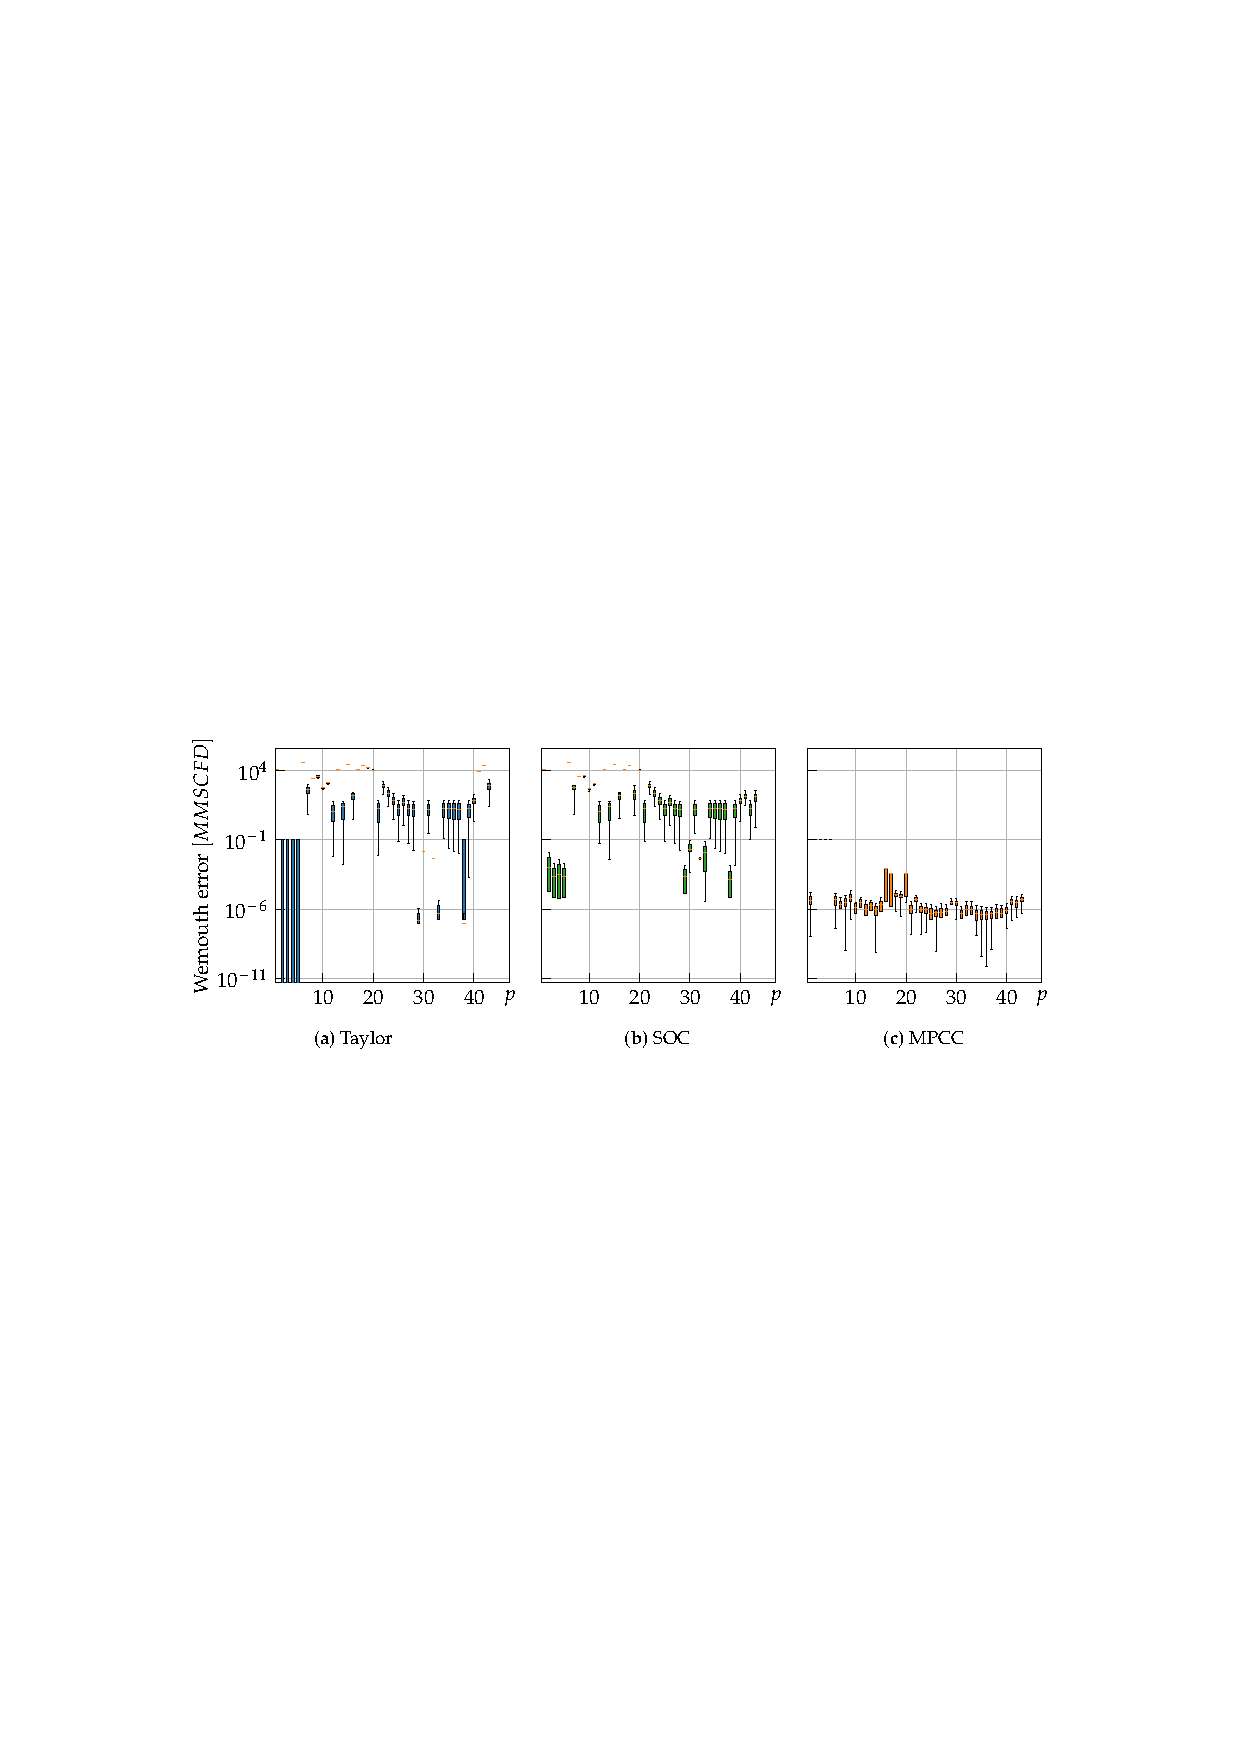
\includegraphics[scale=1.05]{figures/Chapter_MPCC/g004.pdf}
% \end{adjustwidth}
\caption{Weymouth approximation errors for each pipeline $p$ reached by the contrasted approaches in the 118/48 study case.} 
\label{fig:green_test_error}
\end{figure}

\subsection{Case Study III: 96/63 System}

The last case study focuses on the Colombian power system, a complex network comprising 96 nodes ($\left | \mathcal{N}_P \right | = 96 $), 49 generators ($\left | \mathcal{G} \right | = 49 $), 207 transmission lines ($\left | \mathcal{F} \right | = 207 $), and 80 power users ($\left | \mathcal{D} \right | = 80 $). From the 49 generators, 10 are thermal power plants ($\left | \mathcal{I} \right | = 10 $) fed by the natural gas transportation system, including 13 wells ($\left | \mathcal{W} \right | = 13 $), \mbox{48 pipelines} ($\left | \mathcal{P} \right | = 48 $), 14 compressor stations ($\left | \mathcal{C} \right | = 14 $), and 26 consuming users (\mbox{$\left | \mathcal{U} \right | = 26 $}), yielding 63 nodes ($\left | \mathcal{N}_{F} \right | = 63 $). Despite its radial structure, the gas system supports bidirectional flows in its pipelines due to the highly varying demand by thermal power plants influenced by meteorological conditions: On rainy seasons, thermal power plants dramatically reduce their demand; while on dry seasons, a large amount of gas must flow to them. 


Instead of estimating the distributions of the cost function and Weymouth error as in cases 9/8 and 118/48, the 96/63 case validates the Weymouth approximations in an operation case of ten consecutive days ($\left | \mathcal{T} \right | = 10 $) with randomly changing gas extraction costs. Such a complementary validation strategy allows the interconnected system to reduce gas transportation costs by exploiting its single storage station, extending the performance analysis to scheduling scenarios.
\Cref{fig:red_test_cost} illustrates the daily optimized operating cost of the integrated system over the ten-day scheduling horizon for each tested approach. The daily cost values reveal notable similarities between the Taylor series and SOC relaxations. Nonetheless, the MPCC approach yields a 2.7\% more expensive solution, from 8\% cheaper to 12\% more expensive, with a difference standard deviation of 6\%. The above results indicate that the difference between the proposed MPCC and baseline approximations is statistically negligible and will disappear after the empirical corrections.

\begin{figure}[H]
   \hspace{-6pt}  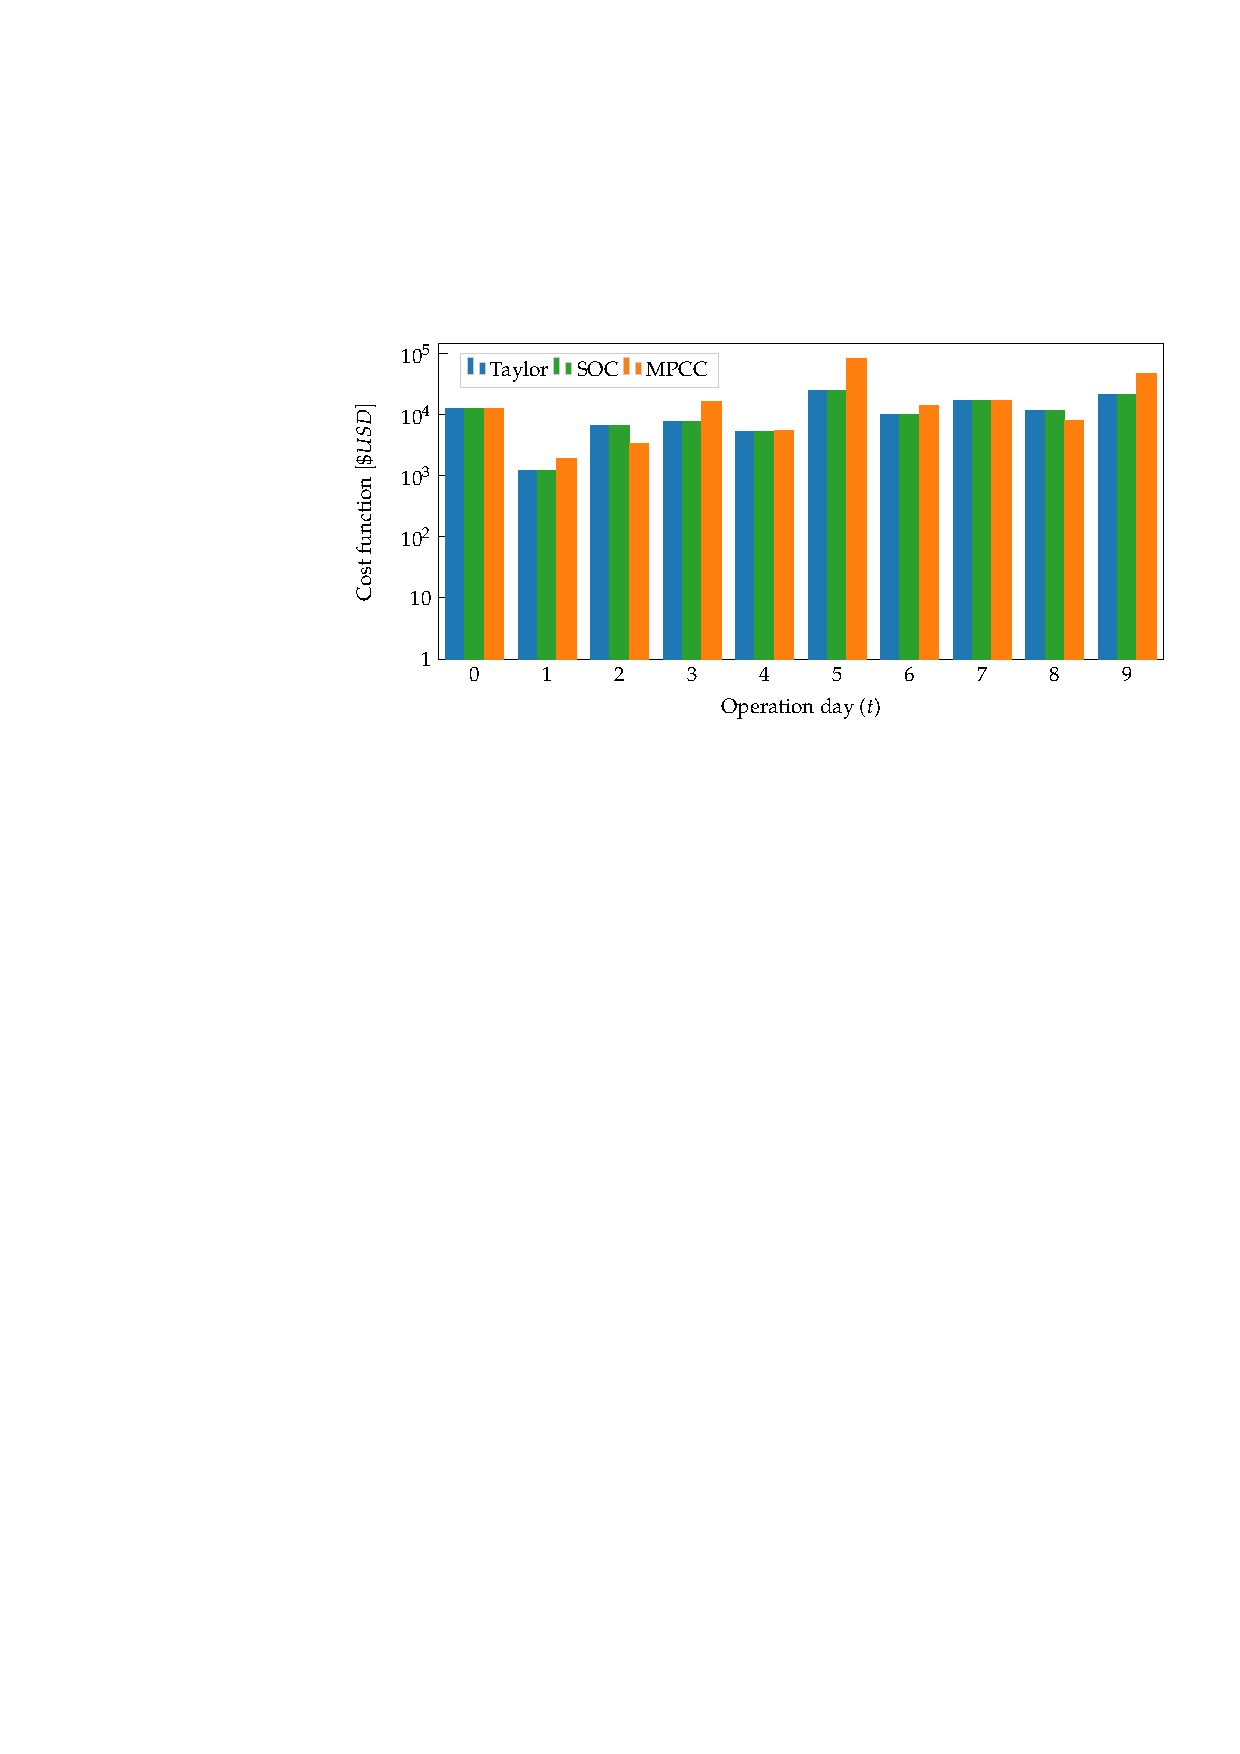
\includegraphics[scale=0.98]{figures/Chapter_MPCC/g005.pdf}
    \caption{Daily operating cost obtained with each of the approaches in the 63-node 96-bus system.}
    \label{fig:red_test_cost}
\end{figure}


Regarding the Weymouth approximation analysis, \Cref{fig:red_test_error} presents the error distribution and its relationship with the gas flow and the scheduled day for Taylor, SOC, and MPCC. Firstly, the error histogram in \Cref{fig:red_test_error}a proves that the proposed MPCC formulation (in green) exhibits superior approximation accuracy to Taylor and SOC for most pipelines and days. Secondly, the scatter plot in~\Cref{fig:red_test_error}b  illustrates the relationship between Weymouth error and gas pipeline flow for each approach. Note that the benchmark techniques of Taylor (blue) and SOC (orange) hold a stationary error regardless of the flow rate. In the case of MPCC (green), the larger the flow rate, the shorter the error dispersion. In addition, despite its large error dispersion at low flow rates, MPCC still delivers much lower errors than benchmark methodologies. Hence, the complementarity constraints improve the error rates of Taylor and SOC and become more reliable for higher gas \mbox{flow rates}.


\begin{figure}[H]
   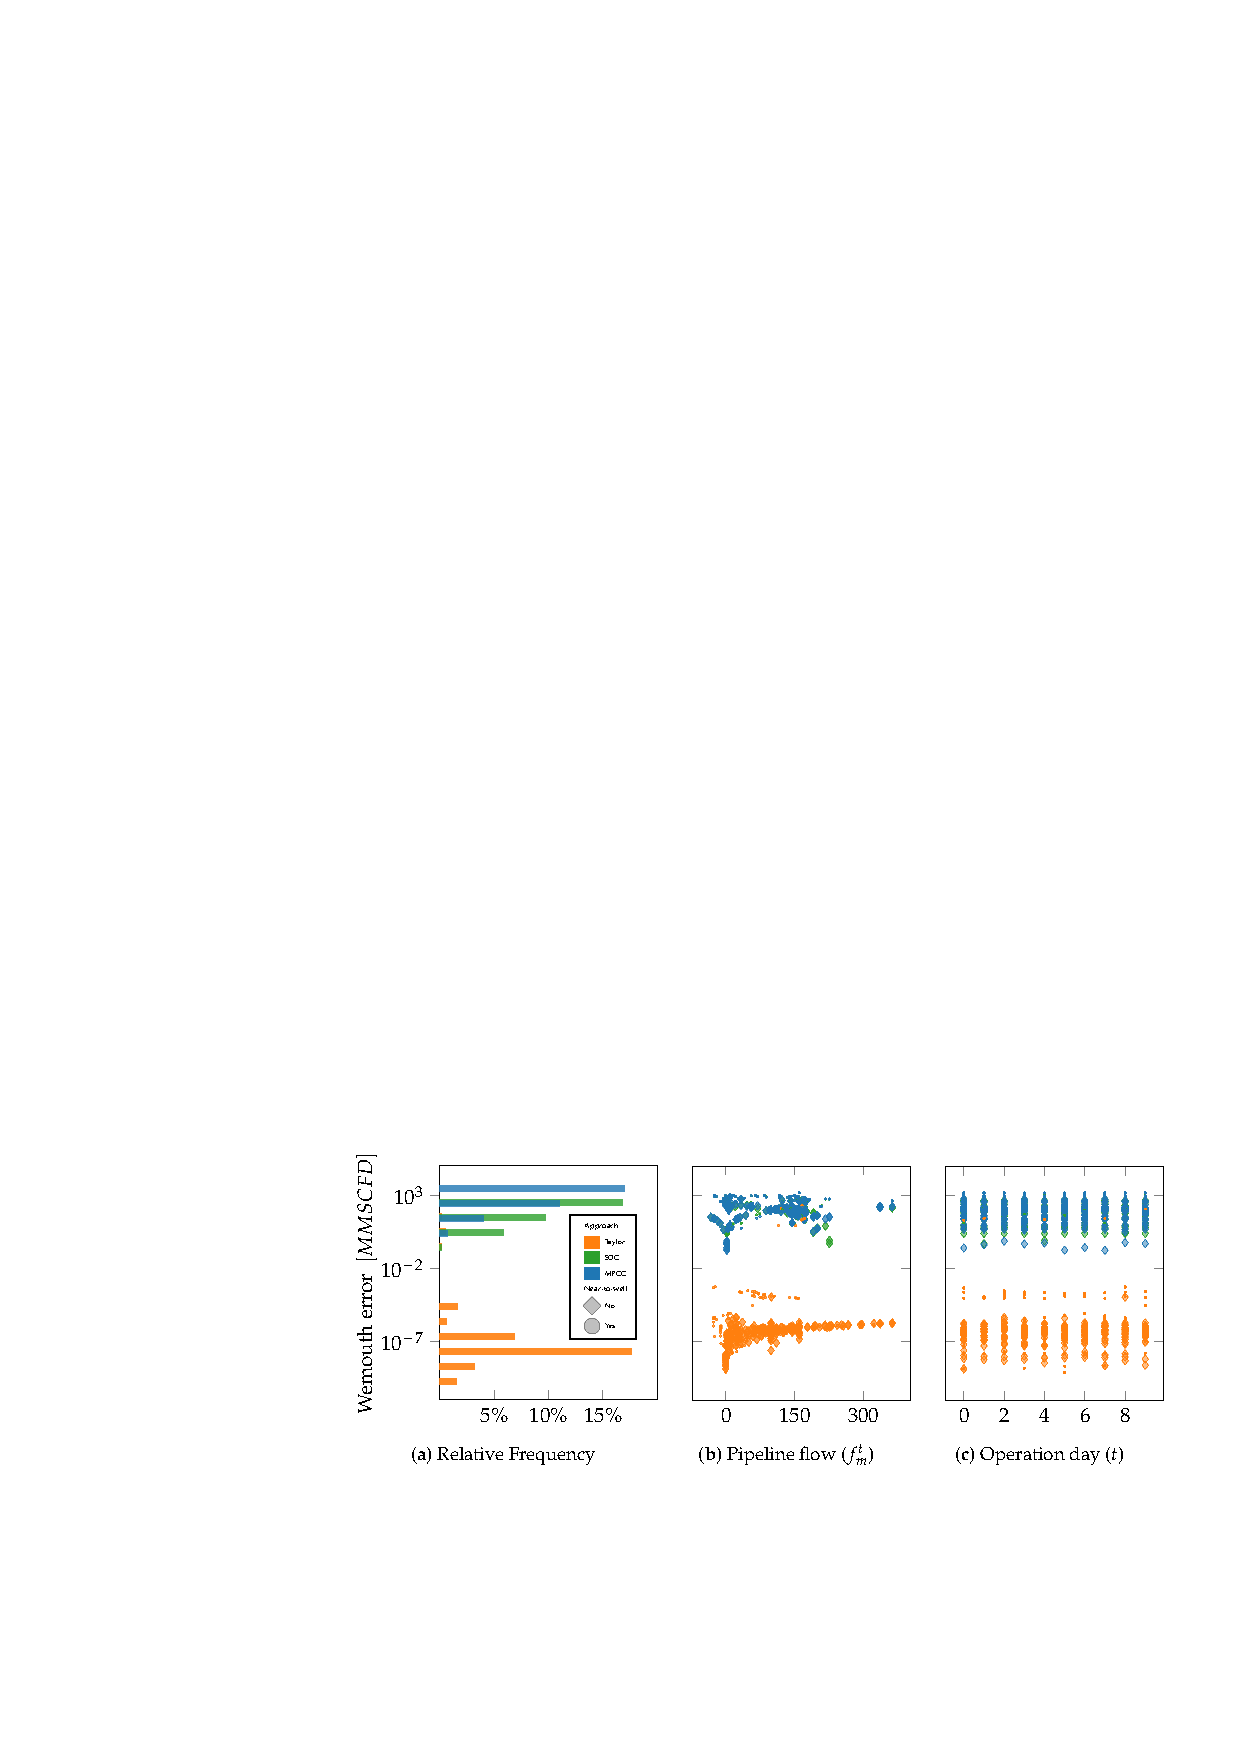
\includegraphics[scale=0.98]{figures/Chapter_MPCC/g006.pdf}
\caption{Weymouth error density on the Colombian case versus the gas flow and operation day.}\label{fig:red_test_error}
\end{figure}

Lastly, \Cref{fig:red_test_error}c suggests independence between the Weymouth error and each scheduled day, with a stationary error distribution for all approximations. Nonetheless, MPCC holds two groups of outlying errors. The higher ones align with typical magnitudes of the benchmark techniques. The second group of errors, lying around $10^{-2}$, corresponds to pipelines connected to injection wells (denoted as dots in \Cref{fig:red_test_heatmaps}c). Since the wells are technically regulated, their fixed injection pressure hampers the flexibility of MPCC for approximating the Weymouth equation.

The heatmaps in \Cref{fig:red_test_heatmaps}c illustrate the output-to-input pressure ratio for each of the \linebreak 14 compressors over the ten days of the scheduled operation. The baseline approaches of Taylor and SOC (\Cref{fig:red_test_heatmaps}a,b) yield constant pressure ratios stemming from an over-relaxation of the Weymouth equation that extends the feasible region to unpractical solutions. In contrast, the MPCC approach in \Cref{fig:red_test_heatmaps}c exhibits day-to-day pressure ratio changes within each compressor. The above is because the complementarity constraints closely align with the gas transport system's real physics, restraining the range of the feasible pressure values to trade off the daily varying injection cost.

\vspace{-4pt}
\begin{figure}[H]

% \begin{adjustwidth}{-\extralength}{0cm}
\centering %% If there is a figure in wide page, please release command \centering
 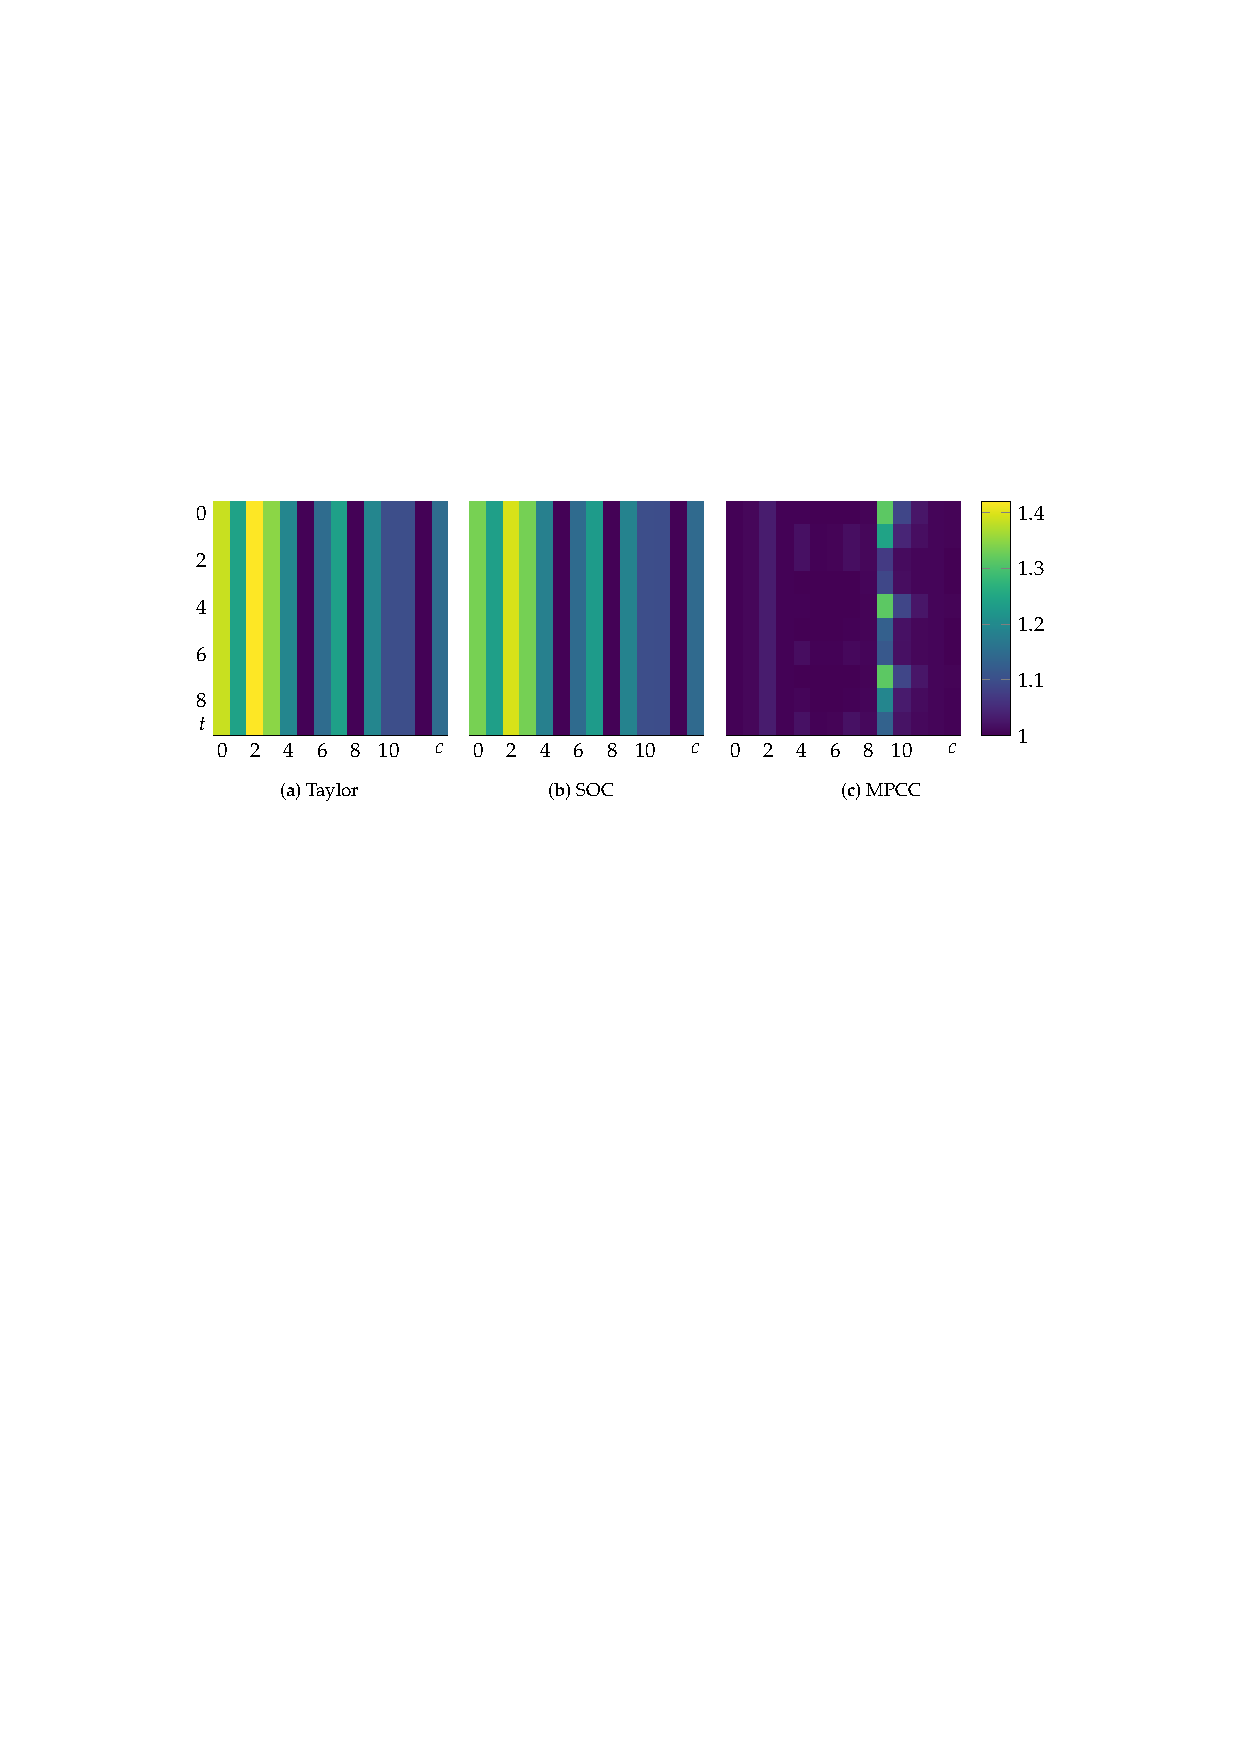
\includegraphics[scale=1.03]{figures/Chapter_MPCC/g007.pdf}
% \end{adjustwidth}
\caption{Output-to-input pressure ratio at the compressor in the  96/63 system. }
\label{fig:red_test_heatmaps}
\end{figure}


As a remark, compressor nine in \Cref{fig:red_test_heatmaps}c reaches large pressure ratios on Days 0, 1, 2, 4, and 7, overlapping with the time instants with the highest approximation errors for MPCC in \Cref{fig:red_test_error}c. A detailed examination of these outcomes detects that compressor nine and the outlying pipeline are the two outputs of a bifurcation, the latter being followed by an injection well. \Cref{fig:96 63partial network} exemplifies that such an interconnection is the sole over the gas network. As a hypothesis, fixing the pressure at the injection well and the flow direction at compressor nine pushes the complementarity constraints to the limits and forces the compressor to augment the pressure ratio to satisfy the forthcoming branch demand.


\begin{figure}[H]
    \centering
    
    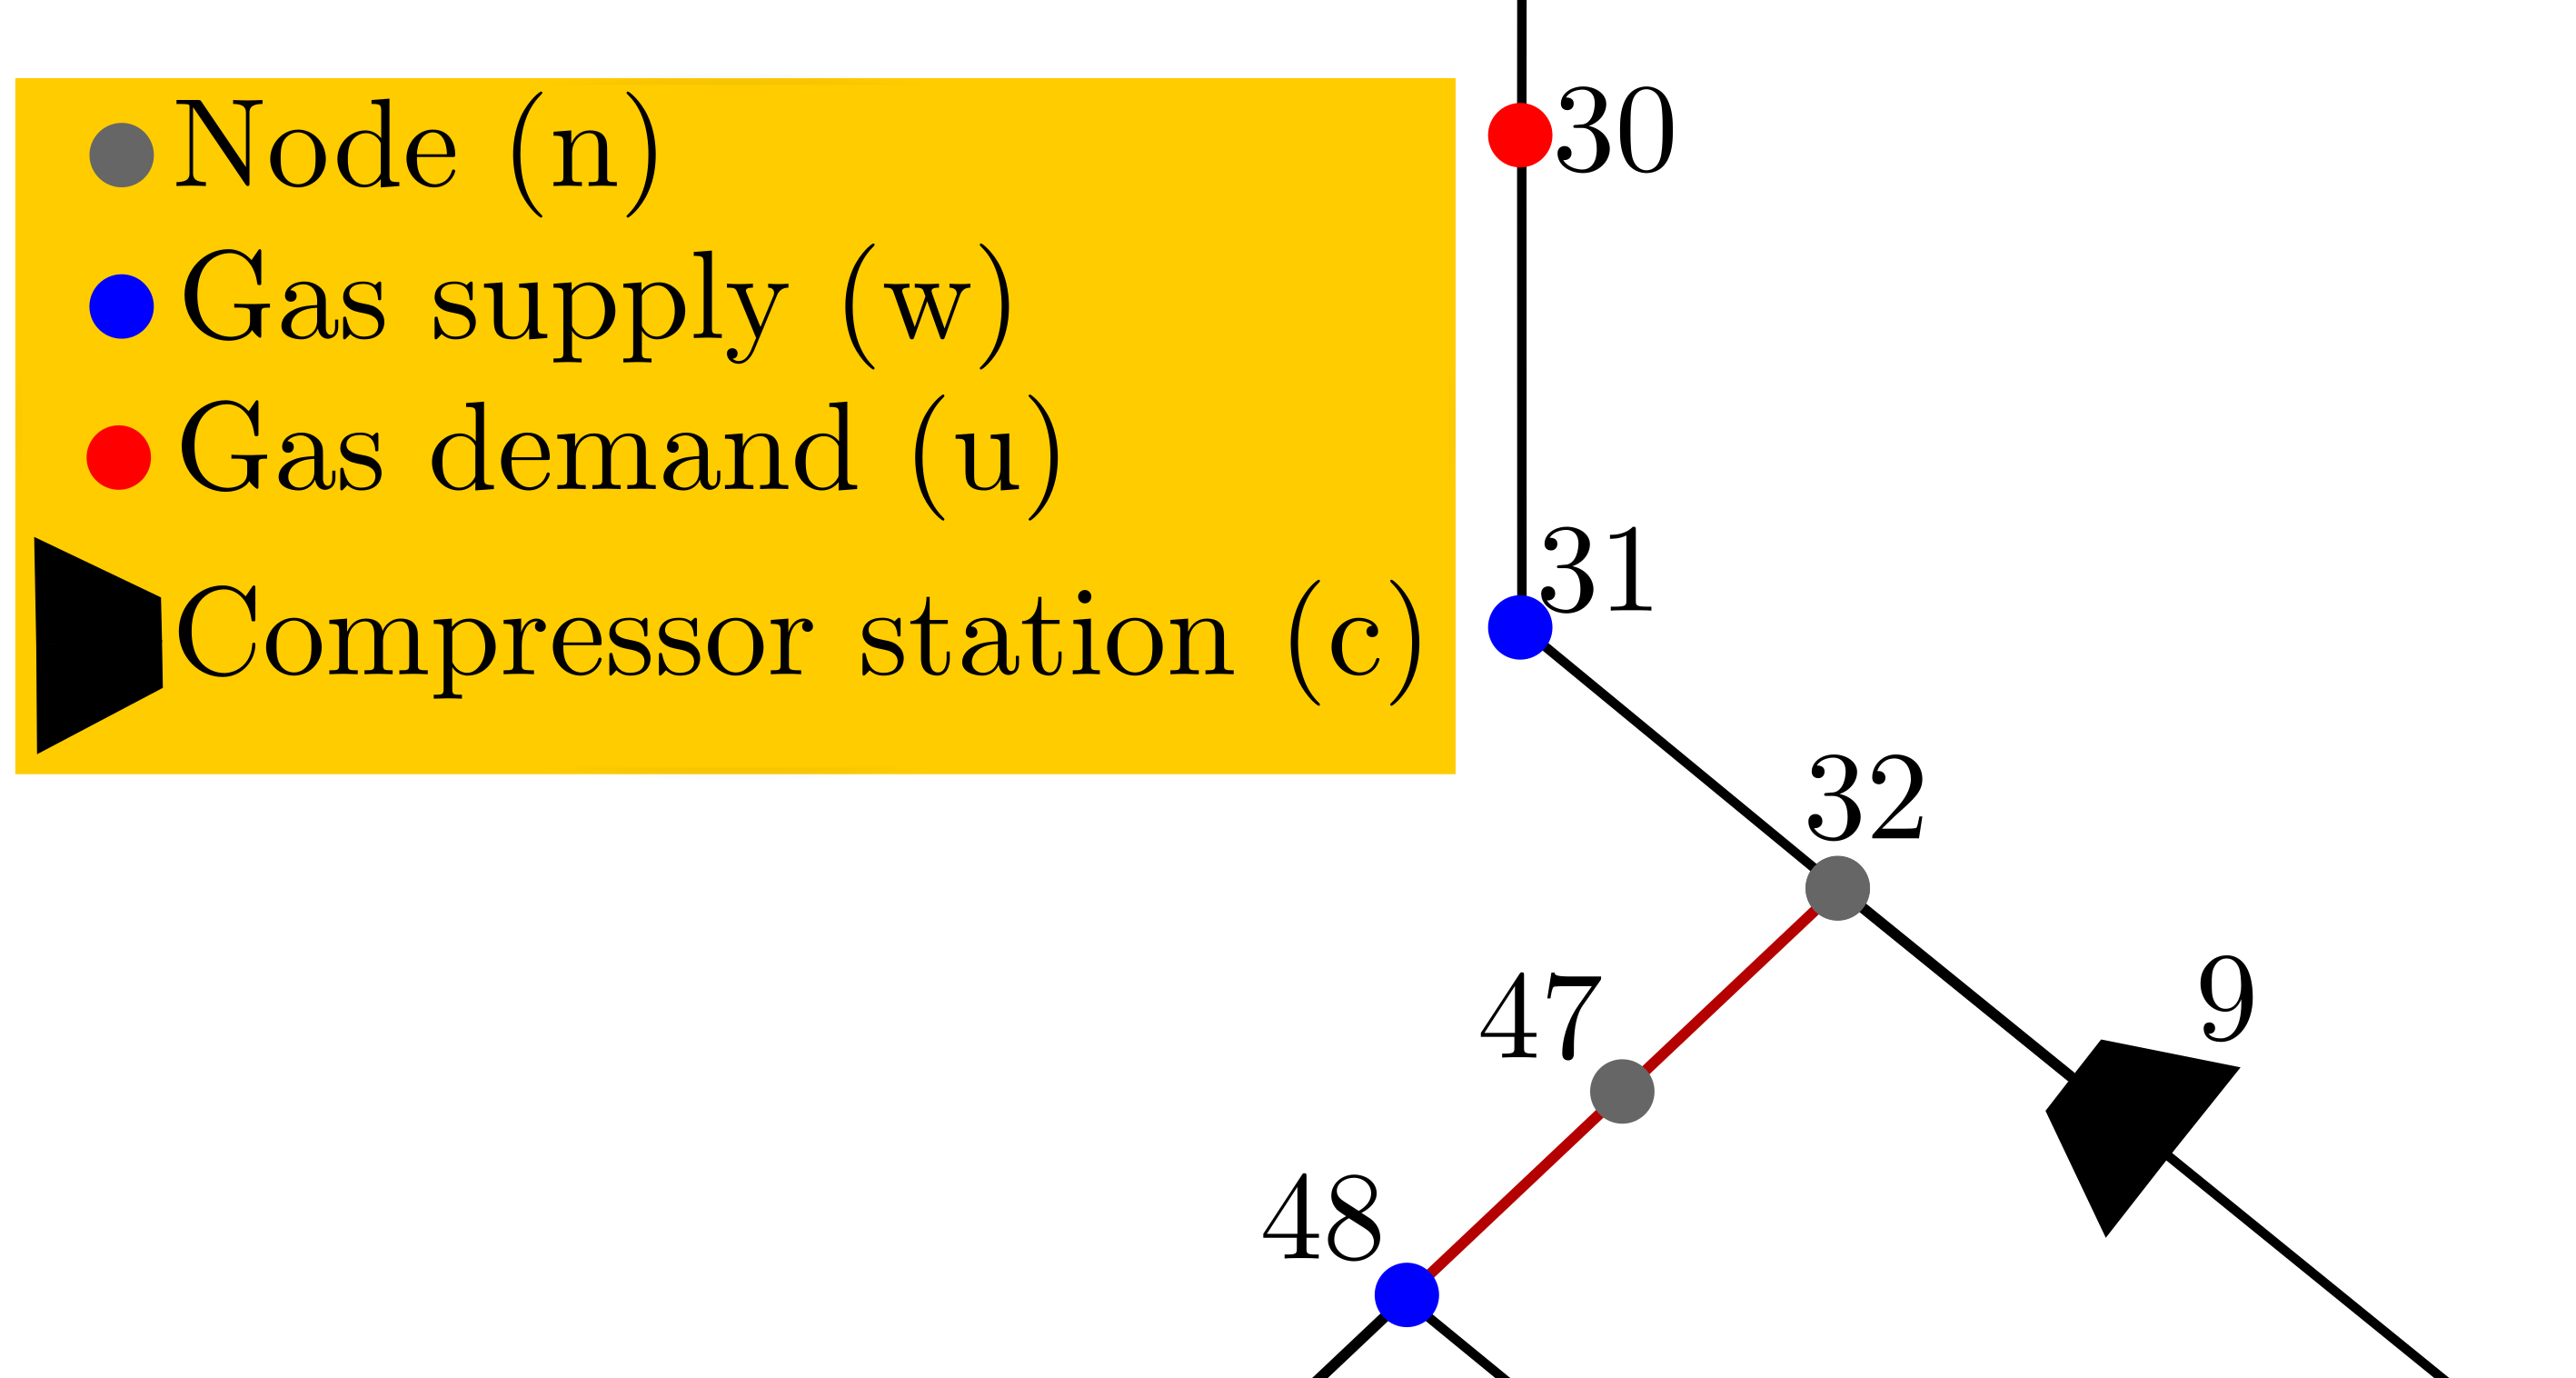
\includegraphics[scale=1.5]{figures/Chapter_MPCC/partial_network}
    \caption{Outlying connection of well-compressor-pipeline on the system 96/63 used in Case Study III.}
    \label{fig:96 63partial network}
\end{figure}

\section{Conclusions} \label{sec: conclusion}

This paper presented a novel approximation for the Weymouth constraint by representing the nonconvex pressure--flow relationship as an MPCC. The MPCC-based formulation significantly benefits the optimization problems in interconnected power and gas systems using binary-behaving continuous variables related to the flow direction, which avoids costly mixed-integer approximations. Additionally, the MPCC inherently captures the complexity in the signum function, resulting in a rigorous approximation of the Weymouth equation.

The validation compared the proposed MPCC approach against the Taylor series and SOC programming approximations on optimizing the operation of interconnected power and gas transport systems. Monte Carlo experiments validated the solution reliability in two well-known case studies, while a ten-day operation planning assessed the scheduling task in a real-world case study.

Regarding cost function, the MPCC approach demonstrated a remarkable ability to balance operational costs effectively. Results on the  9/8 system proved that MPCC converges to the exact cost of Taylor and SOC in small-scale cases. For more complex networks (cases 118/48 and 96/63), MPCC yields higher operational costs than baselines due to the more rigorous Weymouth equation modeling. Nonetheless, the cost differences among approaches lie within reasonable limits and align with the dispatcher's empirical decisions.

In the case of Weymouth approximation, MPCC significantly outperforms Taylor and SOC in the tested cases. In the 118/48 and 96/63 systems, MPCC substantially reduces Weymouth approximation errors, often by several orders of magnitude, compared to traditional linearization and convex relaxation strategies. Such an accuracy improvement becomes crucial in large-scale, complex systems where precise approximation directly influences operational efficiency and system reliability. Hence, the introduced pressure--flow model mathematically benefits the optimization task, asserting its cost-effectiveness at various system scales.

The analysis of the scheduling task in the 96/63 Colombian interconnected system underscores the robustness and reliability of the MPCC approach. Despite the complexities of bidirectional flows and time-varying demand scenarios, MPCC maintains high accuracy levels in Weymouth approximation. Furthermore, the nearly negligible cost differences among approximation approaches establish MPCC as the most robust and reliable approach for short-term operational scheduling.

In conclusion, modeling the Weymouth equation as an MPCC improves the optimization of interconnected gas and power systems by balancing operational costs, minimizing approximation errors, and handling scheduling tasks. These findings establish strong evidence for the practical implementation of MPCC in gas transport optimization, particularly in scenarios demanding high accuracy and reliability in short-term operation scheduling.

Considering the current open issues on energy management, three future research directions may complement this study. Firstly, we propose to adapt MPCC to dynamic system constraints for validation in transient analysis scenarios. The second research direction accounts for the uncertainty in interconnected systems, mainly due to the growing share of low-inertia power sources, such as wind and solar, and potential gas transport failures. Hence, we plan to extend the proposed methodology to stochastic optimization, considering the varying parameters and power sources of interconnected systems. Lastly, we will integrate MPCC with distributed cooperative operation schemes considering multi-agent issues such as the lack of information due to privacy policies~\citep{DING2024123275}.
